\documentclass[]{./tpl/isipfe}
\graphicspath{{./img/}{./}}
\usepackage{acronym}
\usepackage{subfig}
\input{./tpl/new_commands}
\setlength{\parskip}{0pt}
\setlength{\parindent}{0pt}
\makeindex
\usepackage[english]{babel}
\makeindex
\usepackage{tabularx}
\usepackage{booktabs}
\usepackage{float}
\usepackage{mdframed}
\usepackage{xcolor}
\definecolor{fdnavy}{RGB}{0, 32, 96}
\begin{document}
    %============= Config new columns type ==============%
\newcolumntype{L}{>{\raggedright\arraybackslash}}
\newcolumntype{R}{>{\raggedleft\arraybackslash}}
\newcolumntype{C}{>{\centering\arraybackslash}}
%==================================================%

\title{Final Year Project Report}

\author{Youssef BEN ABID \\ Anas YOUNES}

\diplomaName{Information Technology}
\speciality{Information Technology}

%% Encadrant professionnel
\proFramerName{Mr. Khalil Selmi}

%% Encadrant académique
\academicFramerName{Ms. Ines Ben Nasr}

%% Entreprise d'accueil
\companyName{ATOMIC IT}

%% Année universitaire
\collegeYear{2025 - 2026}

%%%%%% Abstracts %%%%%%

%%% AR
\arabicAbstract{هذا العمل يندرج في إطار مشروع ختم الدراسات لنيل الإجازة في تكنولوجيا المعلومات للسنة الجامعية 2025-2026. يتمثل المشروع في تطوير منصة نقل تشاركي تونسية تُدعى "ForsaDrive"، وهي عبارة عن تطبيق ويب وتطبيق جوال يهدفان إلى تسهيل التنقل وتقليل التكاليف وتعزيز المشاركة بين المستخدمين.}

%%% FR
\frenchAbstract{Ce travail s'inscrit dans le cadre du projet de fin d'études pour l'obtention d'une licence en technologie de l'information pour l'année universitaire 2025-2026. Le projet consiste à développer une plateforme tunisienne de covoiturage appelée "ForsaDrive", comprenant une application web et une application mobile visant à faciliter les déplacements, réduire les coûts et encourager le partage entre utilisateurs.}

%%% EN
\englishAbstract{This work is part of the Final Year Project for obtaining a bachelor's degree in Information Technology for the academic year 2025-2026. The project consists of developing a Tunisian carpooling platform called "ForsaDrive", including both a web application and a mobile application, aiming to facilitate transportation, reduce costs, and promote shared mobility among users.}

%% Informations entreprise
\setboolean{wantToTypeCompanyAddress}{true}

\companyEmail{contact@atomicitpro.com}
\companyTel{}
\companyFax{}

\companyAddressAR{قليبية، نابل، تونس}
\companyAddressFR{Kelibia, Nabeul, Tunisia}

    \frontmatter
        
%===== File containing the main cover of the document =====%
%                                                          %
% Copyright (C) ISI - All Rights Reserved                  %
% Proprietary                                              %
% Written by Med Hossam <med.hossam@gmail.com>, April 2016 %
%                                                          %
% @author: HEDHILI Med Houssemeddine                       %
% @linkedin: http://tn.linkedin.com/in/medhossam           %
%==========================================================%

%== It's advised to not modify the content of this file ===%
% To set your information, go to global_config.tex file    %
%==========================================================%

\thispagestyle{cover}%
\newgeometry{bottom=25mm,left=20mm,top=15mm,right=20mm}
\hspace{-47pt}
\begin{minipage}[l]{0.2\columnwidth}
\vspace{6mm}

\includegraphics[width=1.1\columnwidth]{img/image.png}\\
\end{minipage}
\hfill
\begin{minipage}[l]{0.6\columnwidth}
\centering
\footnotesize
\textbf{{Tunisian republic}}\\
\vspace{1.5mm}
\textbf{{MINISTRY OF HIGHER EDUCATION AND SCIENTIFIC RESEARCH\\
GENERAL DIRECTORATE OF TECHNOLOGICAL STUDIES}}\\
\vspace{1.5mm}

\textbf{{Institute of Technological Studies of Kelibia}}
\end{minipage}
\hfill
\begin{minipage}[l]{0.02\columnwidth}
\end{minipage}
\hfill
\begin{minipage}[l]{0.18\columnwidth}
\vspace{6mm}

\includegraphics[width=0.9\columnwidth]{tpl/minister.png}\\
\end{minipage}
\vskip1.5cm

\begin{center}
{\LARGE{\textbf{\textsc{Final Year Project report}}}}\\
\vskip0.5cm
\large


{\textbf{Department \@speciality}}\\
{}
\end{center}

\begin{center}
\textrm{By}\\
\vskip0.3cm
{\ifthenelse{\boolean{isBinomal}}
    {% IF TRUE
        \begin{center}
            \large\textbf{\@author}~~~~~ et ~~~~~
            \large\textbf{\@secondAuthor}
        \end{center}
    }
    {\Large\textbf{\@author}}% FALSE
}
\vskip12mm

\definecolor{isiBlue}{RGB}{31, 78, 121}

\begin{changemargin}{-9mm}{0cm}
\begin{minipage}[l]{1.1\columnwidth}
\begin{tcolorbox}[colframe=isiBlue,colback=white,boxrule=0pt,toprule=3pt,bottomrule=3pt,arc=0pt,top=0mm,right=0mm,left=0mm,bottom=0mm,boxsep=0.5mm]{
    \begin{tcolorbox}[colframe=isiBlue,colback=white, boxrule=0pt,toprule=1pt,bottomrule=1pt,arc=0pt,enlarge bottom by=-0.9mm, auto outer arc]
        \centering
        {\huge\textbf{\@title}}
    \end{tcolorbox}
}
\end{tcolorbox}
\end{minipage}
\end{changemargin}

\end{center}
\vskip8mm%

\begin{center}
\large
\begin{minipage}[c]{0.28\columnwidth}
Professional Supervisor:\\
Academic Supervisor:
\end{minipage}
\hfill
\begin{minipage}[c]{0.42\columnwidth}
\textbf{\@proFramerName}\\
\textbf{\@academicFramerName}
\end{minipage}
\hfill
\begin{minipage}[c]{0.26\columnwidth}
\@proFramerSpeciality
\@academicFramerSpeciality
\end{minipage}
\end{center}
\vskip10mm

\begin{center}
\large
Made within \@companyName\\
\vskip0.3cm
\begin{figure}[h]
\centering
{\color{isiBlue}{\fboxrule=2.5pt\fbox{
\includegraphics[width=0.3\columnwidth]{img/Company_Logo.png}}}}
\end{figure}
\end{center}

        \setcounter{page}{1}
        \thispagestyle{frontmatter}
        \chapter*{Acknowledgments}
\begin{center}

First, we would like to express our sincere gratitude to \textbf{Ms. Houda Toukabri}, Head of the IT Department at the Higher Institute of Technological Studies of Kelibia, for her guidance and for providing a supportive academic environment. \\

\vspace{0.5cm}

\parindent=1.5em We would like to extend our deepest thanks to \textbf{Ms. Ines Ben Nasr}, our academic supervisor, for her valuable guidance, continuous support, and constructive feedback throughout this project. \\

\vspace{0.5cm}

\parindent=1.5em We also wish to thank \textbf{Mr. Khalil Selmi}, our professional supervisor at \textbf{ATOMIC IT}, for giving us the opportunity to carry out this internship within his company, as well as for his availability, professionalism, and insightful advice. \\

\vspace{0.5cm}

\parindent=1.5em Finally, we would like to thank all \textbf{our professors at ISET Kelibia} who contributed to our education and training. Please accept our sincere appreciation.

\end{center}

\begin{flushright}
    \LARGE Youssef BEN ABID \\
    \LARGE Anas YOUNES
\end{flushright}
        \thispagestyle{frontmatter}

        \setcounter{secnumdepth}{3}
        \setcounter{tocdepth}{2}
        \dominitoc

        \selectlanguage{english}
        \tableofcontents
        \adjustmtc
        \thispagestyle{frontmatter}
        \foreignlanguage{english}{\listoffigures}
        \thispagestyle{frontmatter}

        \selectlanguage{french}

    \mainmatter
        \chapter*{General Introduction}
\addcontentsline{toc}{chapter}{General Introduction}
\markboth{General Introduction}{}

Mobility is one of the most basic conditions of modern economic and social life. Access to reliable transportation determines whether students reach their universities on time, whether workers can take a job in another city, and whether families can maintain regular contact across long distances. In Tunisia, however, this everyday need collides with a transportation system that has not kept pace with the growth of the population or with the geographic distribution of universities, industrial zones, and tourist regions. Public transport is often overcrowded and irregular, fuel prices have risen steadily, and inter-city travel remains expensive and time-consuming for those who do not own a vehicle.

Carpooling has emerged worldwide as a natural answer to this kind of imbalance. By matching drivers who already plan a trip with passengers who are heading in the same direction, it transforms unused seats into a shared resource, reduces the cost of mobility for both sides, and lowers the environmental impact of individual driving. In Tunisia, the demand for such a service is clearly present: thousands of trips between cities such as Tunis, Sfax, Sousse, and the smaller towns of the coast and the interior are organized every week. The supply, however, remains almost entirely informal, scattered across Facebook groups, private messages, and word-of-mouth contacts.

This informal organization carries real consequences. There is no verification of identity, no record of payment, no structured search, and no mechanism to evaluate a driver or a passenger after a trip. International platforms such as BlaBlaCar offer a more structured experience, but their adoption in Tunisia is held back by payment models that do not match local habits, by interfaces that are not localized, and by a user base that is too small to ensure frequent matches on the most requested national routes. The result is a paradoxical situation: a strong demand for shared mobility coexists with the absence of a digital tool truly designed for the country.

It is precisely this gap that the present project addresses. \textbf{ForsaDrive} is a carpooling platform conceived from the start for the Tunisian context. It is built as a unified ecosystem composed of a web application, a mobile application, and a shared backend, so that the same business rules apply regardless of the device used. The platform supports the complete lifecycle of a shared trip: account creation, identity and student verification, ride publication, search and booking, in-app communication, payment with a fifty-percent prepayment that confirms the booking, ratings, and complaint handling. It also introduces features that respond to specific local realities, including a verified student status that grants an automatic fifty-percent discount, support for cash payment of the remaining balance, and an interface designed for English, French, and Arabic users. The project was carried out within the company \textbf{ATOMIC IT}, which provided the professional environment, the technical supervision, and the methodological framework needed to take the idea from a sketch to a structured deliverable.

The remainder of this report is organized into five chapters. The first chapter presents the host organization and the general framework of the project, including a critical analysis of the current transportation situation in Tunisia and the motivations that led to ForsaDrive. The second chapter surveys existing solutions, identifies the actors of the system, formalizes the functional and non-functional requirements, and explains the agile methodology followed during the internship. The third chapter covers the conception of the platform: the general architecture, the most representative use cases, the dynamic behavior through sequence and activity diagrams, and the structural design through a class diagram and a relational schema. The fourth chapter describes the realization of the web platform, from the development environment and the technology stack to the main delivered interfaces. The fifth chapter presents the mobile application built with Flutter, the mobile-specific features it adds, and the testing strategy applied across the full platform. The report closes with a general conclusion that summarizes what was achieved, identifies the remaining limitations, and outlines the directions for future work.
        \clearpage

        %=============================================================================
%  CHAPTER 1 — PROJECT FRAMEWORK
%=============================================================================
\chapter{Project Framework}

\clearpage
\section*{Introduction}

Before describing the technical work carried out on ForsaDrive, it is necessary to situate the project in its concrete context. This chapter therefore presents the host organization within which the internship was conducted, examines the current state of mobility in Tunisia and the limits of the solutions that users currently rely on, and finally states the motivations and objectives that led to the development of the platform. The chapter closes with an outline of the proposed solution, which serves as the bridge towards the analysis of requirements presented in the next chapter.


\section{Study of the Host Organization}

\subsection{Presentation of ATOMIC IT}

ATOMIC IT is an information technology engineering services company specialized in the design and development of digital solutions. Its team brings together engineers, technicians, and IT specialists who work primarily on web and mobile development. The company assists its clients in the full lifecycle of their software projects, from the initial expression of needs to the deployment and maintenance of the delivered system.

Beyond pure development, ATOMIC IT positions itself as a partner that helps its clients translate business requirements into reliable digital tools. It relies on modern technologies and on programming environments such as Windows and Linux, the .NET and Java ecosystems, and the major mobile platforms (Android and iOS). This breadth of expertise allows the company to work on a wide range of projects, from institutional websites to platforms with significant business logic such as the one developed during this internship.

\subsection{General Information about ATOMIC IT}

Table~\ref{tab:atomic_info} summarizes the main administrative information about the host organization.

\begin{table}[H]
\centering
\caption{General information about ATOMIC IT}
\label{tab:atomic_info}
\begin{tabular}{|l|p{9cm}|}
\hline
\textbf{Address}      & Arab League Street, Kélibia, Nabeul Governorate \\
\hline
\textbf{Phone Number} & +216 55 343 224 \\
\hline
\textbf{Activity}     & Web and mobile development, software engineering, and digital consulting \\
\hline
\textbf{Director}     & Mr. Khalil Selmi \\
\hline
\textbf{Core focus}   & Design and delivery of responsive web platforms and mobile applications adapted to client needs \\
\hline
\end{tabular}
\end{table}

\subsection{Services Offered by ATOMIC IT}

The company structures its activity around four main services that complement each other.

\begin{description}[noitemsep]
    \item[Website Creation.] Design of responsive and customized websites, with attention to performance, accessibility, and scalability. The company adapts the technical stack to the client's profile, whether the goal is a content-driven site or a more dynamic interface.
    \item[Web Engineering.] Development of more complex platforms such as e-commerce systems, community platforms, and data-driven applications. This service covers backend architecture, database modeling, and the integration of third-party components such as payment gateways or notification services.
    \item[Web Marketing.] Support in the definition of digital marketing strategies. The company assists its clients in the choice of channels, the structuring of campaigns, and the alignment of online communication with measurable business objectives.
    \item[Search Engine Optimization.] Improvement of the visibility of websites in search engines through keyword strategies, indexing, and the application of best practices in technical and content SEO.
\end{description}

The internship took place primarily within the engineering activity of the company, since ForsaDrive belongs to the family of data-driven platforms with significant business logic.

\subsection{Organizational Chart of ATOMIC IT}

The internal organization of ATOMIC IT is deliberately flat and oriented towards short communication paths between decision making and execution. Figure~\ref{fig:atomic_org} presents the simplified organizational chart of the company.

\begin{figure}[H]
    \centering
    
\includegraphics[width=0.8\textwidth]{image.png}
    \caption{Organizational chart of ATOMIC IT}
    \label{fig:atomic_org}
\end{figure}

At the top level, the chief executive officer supervises strategic decisions, validates project directions, and represents the company with its clients. The development teams handle the technical implementation, while interns contribute to ongoing projects under the supervision of senior developers. This structure favors quick feedback loops, which proved beneficial during the internship since the validation of design choices on ForsaDrive could take place without intermediate delays.

\subsection{Internship Framework}

The internship was carried out within the development team of the company, in coordination with both frontend and backend developers. The work followed an agile Scrum approach, with daily stand-up meetings inside the team and weekly reviews with the supervising engineer. This rhythm allowed a continuous validation of progress and gave the opportunity to adjust priorities as the project advanced.

The two interns who collaborated on ForsaDrive worked on the same shared application rather than on two independent products. The work was therefore distributed by functional modules and by sprints, not by a strict separation between web and mobile responsibilities. This organization made it possible to keep the business logic consistent across the two interfaces and to share the design effort on the most sensitive parts of the system, such as authentication, the booking flow, and the payment logic.


\section{Critical Study of the Existing Situation}

\subsection{General Context}

Mobility plays a central role in economic activity, education, and social interaction. In Tunisia, transportation conditions every aspect of daily life, from the choice of a university to the feasibility of a job offer in another governorate. Yet, the available means of transportation suffer from structural limitations that make travel both expensive and unpredictable. Public transport between cities is often overcrowded and irregular, the road network does not always serve secondary towns with the same frequency as the main corridors, and private cars travel every day with empty seats that no system currently helps to fill.

This situation places a particular burden on students and young professionals, who travel frequently but have limited budgets. It is in this segment that the demand for a reliable and affordable shared mobility service is the most visible.

\subsection{Analysis of Current Limitations}

The mobility solutions currently available in Tunisia each address part of the problem but leave significant gaps. Public transport remains the cheapest option, but its capacity is limited and its schedule does not match the flexibility that students or workers often need. Informal carpooling, which is mostly organized through Facebook groups and private messaging, fills part of the demand but does so without any structure: there is no verification of the identity of drivers or vehicles, no traceability of payments, no centralized search, and no mechanism to rate or report a user after a trip. International applications such as Bolt or inDrive operate on a ride-hailing model designed for short urban trips, and their pricing logic is not adapted to long-distance carpooling. International carpooling platforms such as BlaBlaCar are technically suitable but suffer from a low local adoption, partly because their payment methods, customer support, and user base are not aligned with the realities of the Tunisian market.

Several recurring weaknesses can be summarized as follows:

\begin{itemize}[noitemsep]
    \item Public transport suffers from delays, overcrowding, and insufficient geographic coverage.
    \item Existing international platforms are not fully adapted to local realities such as payment methods, identity verification, or regional mobility patterns.
    \item Informal ride-sharing lacks trust mechanisms such as identity checks, ratings, or secure communication channels.
    \item Private vehicles are underutilized, with many empty seats during daily and weekly trips.
    \item No centralized solution offers a structured advantage to students, who form a large part of the inter-city travel demand.
\end{itemize}

These limitations highlight the absence of a structured, secure, and locally adapted system for shared mobility.

\subsection{Problem Statement}

The analysis of the existing situation can be condensed into a single observation:

\begin{quote}
\textit{Tunisia lacks a secure, affordable, and well-structured digital ride-sharing solution that is adapted to local payment habits, available on both web and mobile, and capable of building genuine trust between drivers and passengers.}
\end{quote}

The challenge is therefore not to invent a new concept, but to adapt the proven model of carpooling to the specific constraints of the Tunisian context.

\subsection{Project Motivation}

The motivation behind ForsaDrive is at the same time social, economic, and technical. On the social side, the project aims to make mobility more accessible to populations whose budget excludes private taxis and whose schedule is not always compatible with public transport, particularly students. On the economic side, the platform contributes to a better use of an existing resource, namely the empty seats of vehicles already on the road, which translates into shared savings for drivers and passengers. On the technical side, the project offers the opportunity to design a complete software ecosystem, articulating a web application, a mobile application, and a shared backend around a coherent business logic.

\subsection{Project Objectives}

The general objective of the project is the design and the implementation of a complete carpooling platform adapted to the Tunisian context. This general objective is broken down into the following specific objectives:

\begin{enumerate}[noitemsep]
    \item Develop a web platform that supports the management of rides and the administration of the system.
    \item Build a mobile application that covers the daily interactions of drivers and passengers.
    \item Provide a unified backend that exposes a single set of business rules to both clients.
    \item Integrate trust mechanisms based on identity verification, ratings, and complaint handling.
    \item Implement a wallet-based payment flow with a fifty-percent prepayment that confirms the booking and a remaining balance settled in cash during the trip.
    \item Offer a verified student status that grants an automatic discount on eligible trips.
    \item Ensure security, scalability, and maintainability throughout the architecture.
\end{enumerate}

\subsection{Proposed Solution}

ForsaDrive is designed as an integrated ecosystem composed of three coordinated components: a web application, a mobile application, and a shared backend. The platform supports the complete carpooling lifecycle, from registration to post-trip evaluation. A driver can publish a trip with its origin, destination, date, price, and number of available seats. A passenger can search for trips, filter results, consult the profile of the driver, book one or several seats, and confirm the booking through a fifty-percent prepayment. After the trip, both parties can rate each other, and any incident can be reported to the administration through a dedicated complaint channel.

The originality of the platform lies in the careful adaptation of every feature to the local context: the payment flow combines an online prepayment with a cash settlement, in line with the way Tunisian users currently handle informal carpooling; the student status is verified through documents or a university email, which makes the discount both accessible and auditable; and the interface is designed to support the languages effectively used by the target population. These choices, which are detailed in the following chapters, are what distinguish ForsaDrive from the international platforms that have so far failed to gain a strong foothold in the country.


\section*{Conclusion}

This chapter introduced the host organization, presented the structural limits of the current transportation situation in Tunisia, and stated the motivations that led to the development of ForsaDrive. It also formulated the general and specific objectives of the project and outlined the proposed solution at a high level. The next chapter translates this general framework into a precise specification: it analyzes the existing competing solutions in more detail, formalizes the actors of the system, and lists the functional and non-functional requirements that the platform must fulfill.
        \clearpage

        %=============================================================================
%  CHAPTER 2 — ANALYSIS AND SPECIFICATION OF REQUIREMENTS
%=============================================================================
\chapter{Analysis and Specification of Requirements}

\clearpage
\section*{Introduction}

The previous chapter established the context of the project and stated the high-level objectives of ForsaDrive. The present chapter takes the analysis one step further by clarifying, in a structured way, who the platform is for, what it must do, and what quality attributes it must respect. The reasoning starts with a comparative review of the mobility solutions on which Tunisians currently rely, ranging from informal social-media groups to international ride-hailing applications. It continues with the description of the development methodology adopted throughout the internship, the identification of the actors of the system, and the listing of the functional and non-functional requirements. The chapter closes with a global use case diagram that summarizes the scope of the platform and prepares the conception phase presented in the next chapter.


\section{Study of Existing Solutions}

Before designing ForsaDrive, it was essential to understand how Tunisians currently organize shared trips, both through formal applications and through informal channels. This step served two complementary purposes: it allowed an objective measure of the gaps left by existing tools and it informed several design decisions presented later, such as the combination of online prepayment and cash settlement.

\subsection{Informal Carpooling through Social Media}

A large share of carpooling activity in Tunisia takes place outside any structured platform. Facebook groups such as \textit{Covoiturage Tunisie}, \textit{Covoiturage Tunis--Sfax}, and regional groups dedicated to specific universities are among the most active channels. Trips are published as simple posts, and passengers contact drivers through private messages or phone calls.

While this informal system genuinely meets part of the demand, it suffers from several structural weaknesses:

\begin{itemize}[noitemsep]
    \item There is no verification of the identity of the driver or of the vehicle.
    \item Payments are handled entirely offline, with no trace of the transaction.
    \item Trip information is scattered across several groups, and no real filtering or sorting is possible.
    \item Cancellations and no-shows are frequent, since neither party has any concrete commitment.
    \item There is no rating system, which forces passengers to rely solely on the comments left under each post.
\end{itemize}

This mode of organization is tolerated rather than regulated, and its very popularity illustrates how strong the demand is for a structured digital alternative.

\begin{figure}[H]
    \centering
    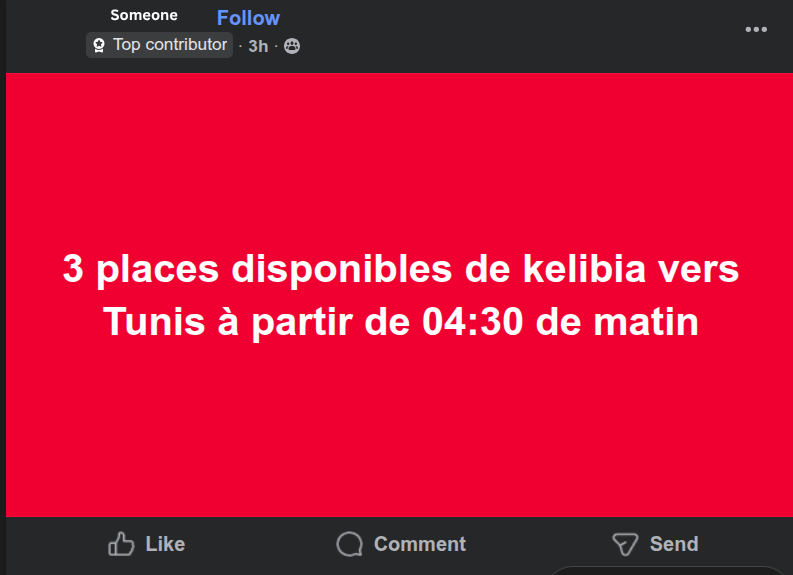
\includegraphics[width=0.7\textwidth]{Post covoiturage.png}
    \caption{Example of an informal carpooling post on a Facebook group}
    \label{fig:facebook_carpooling}
\end{figure}

\subsection{International Ride-Hailing Applications}

Several international ride-hailing applications are currently active on the Tunisian market. Although they are not carpooling platforms in the strict sense, they are often mentioned by users as alternatives for point-to-point travel, which justifies their inclusion in this comparative study.

\subsubsection{inDrive}
inDrive is built on a fare-negotiation model: the passenger proposes a price and drivers can accept the offer or counter-offer. The application is mainly used inside cities such as Tunis, Sousse, and Sfax. However, inDrive is not designed for long-distance travel. Its pricing logic becomes impractical for inter-city routes, and drivers have very little incentive to accept negotiated long trips at a price they cannot adjust based on the number of passengers sharing the vehicle.

\begin{figure}[H]
    \centering
    
\includegraphics[width=0.3\textwidth]{img/indrive.png}
    \caption{inDrive logo}
    \label{fig:indrive_logo}
\end{figure}

\subsubsection{Bolt}
Bolt operates as a classic ride-hailing service with fixed, algorithmic pricing. It is widely used for short urban trips, but it offers no mechanism for sharing a vehicle between passengers heading in the same direction, and its fares rise sharply on longer journeys, which excludes inter-city carpooling from its use cases.

\begin{figure}[H]
    \centering
    
\includegraphics[width=0.3\textwidth]{img/bolt_logo.png}
    \caption{Bolt logo}
    \label{fig:bolt_logo}
\end{figure}

\subsubsection{Uber}
Uber has only a limited presence in Tunisia and is essentially absent from the inter-city segment. For the use cases targeted by ForsaDrive, it is therefore not a realistic alternative.

\subsection{International Carpooling Platforms}

BlaBlaCar is the most well-known carpooling platform internationally and is also used, although on a modest scale, in Tunisia. It offers a structured experience built around verified profiles, integrated payments, and ratings. Its adoption in Tunisia, however, remains low for reasons that have little to do with the quality of the platform itself: payment methods are mostly limited to international cards, customer support operates in foreign languages, and the local user base is too small to ensure frequent matches on the most requested national routes. As a result, the value of the network — which is the main strength of carpooling platforms — is significantly reduced in the Tunisian context.

\begin{figure}[H]
    \centering
    
\includegraphics[width=0.3\textwidth]{img/blablacar.png}
    \caption{BlaBlaCar logo}
    \label{fig:blablacar_logo}
\end{figure}

\subsection{Comparative Table}

Table~\ref{tab:comparison_existing} summarizes the main characteristics of the solutions reviewed above and contrasts them with the features targeted by ForsaDrive.

\begin{table}[H]
\centering
\caption{Comparison of existing solutions with ForsaDrive}
\label{tab:comparison_existing}
\begin{tabular}{|l|c|c|c|c|c|}
\hline
\textbf{Criterion}       & \textbf{Facebook} & \textbf{inDrive} & \textbf{Bolt} & \textbf{BlaBlaCar} & \textbf{ForsaDrive} \\
\hline
Identity verification    & No  & Partial & Yes & Yes & Yes \\
\hline
In-app payment           & No  & No      & Yes & Yes & Yes \\
\hline
Long-distance rides      & Yes & No      & No  & Yes & Yes \\
\hline
Rating system            & No  & Yes     & Yes & Yes & Yes \\
\hline
Adapted to local context & Yes & Partial & Partial & No & Yes \\
\hline
Student discount         & No  & No      & No  & No & Yes \\
\hline
Wallet-based balance     & No  & No      & No  & No & Yes \\
\hline
\end{tabular}
\end{table}

The analysis shows that no existing option simultaneously offers the local fit of informal channels and the reliability of structured platforms. ForsaDrive is positioned precisely in this gap, combining the familiarity of practices that Tunisian users already adopt with the structure, security, and trust mechanisms that international platforms have demonstrated elsewhere.


\section{Development Methodology}

\subsection{Choice of an Agile Approach}

Given the scope of the project, which combines a web application, a mobile application, and a shared backend, a sequential approach such as the waterfall model was rapidly ruled out. Several reasons supported this decision. First, the requirements were expected to evolve as the design progressed, which is typical for a platform whose features have direct counterparts in the daily life of the target users. Second, the project required iterative feedback with the supervising team at ATOMIC IT in order to validate design choices step by step. Third, the team was small and the schedule short, two conditions under which the lightness of an agile process is a clear advantage over the heavier ceremonies of more formal methodologies. The \textbf{Scrum} framework was therefore selected as the development methodology of the project.

\subsection{The Scrum Framework}

Scrum organizes the work into short iterations called sprints, each of which produces a usable increment of the product. Every sprint is planned at the beginning, reviewed at the end, and followed by a short retrospective whose role is to identify what worked, what did not, and which adjustments to apply during the next iteration. Three roles structure the process: the \textit{Product Owner}, who represents the client and maintains the prioritized backlog; the \textit{Scrum Master}, who facilitates the process and removes blocking issues; and the \textit{Development Team}, which builds the increment.

\begin{figure}[H]
    \centering
    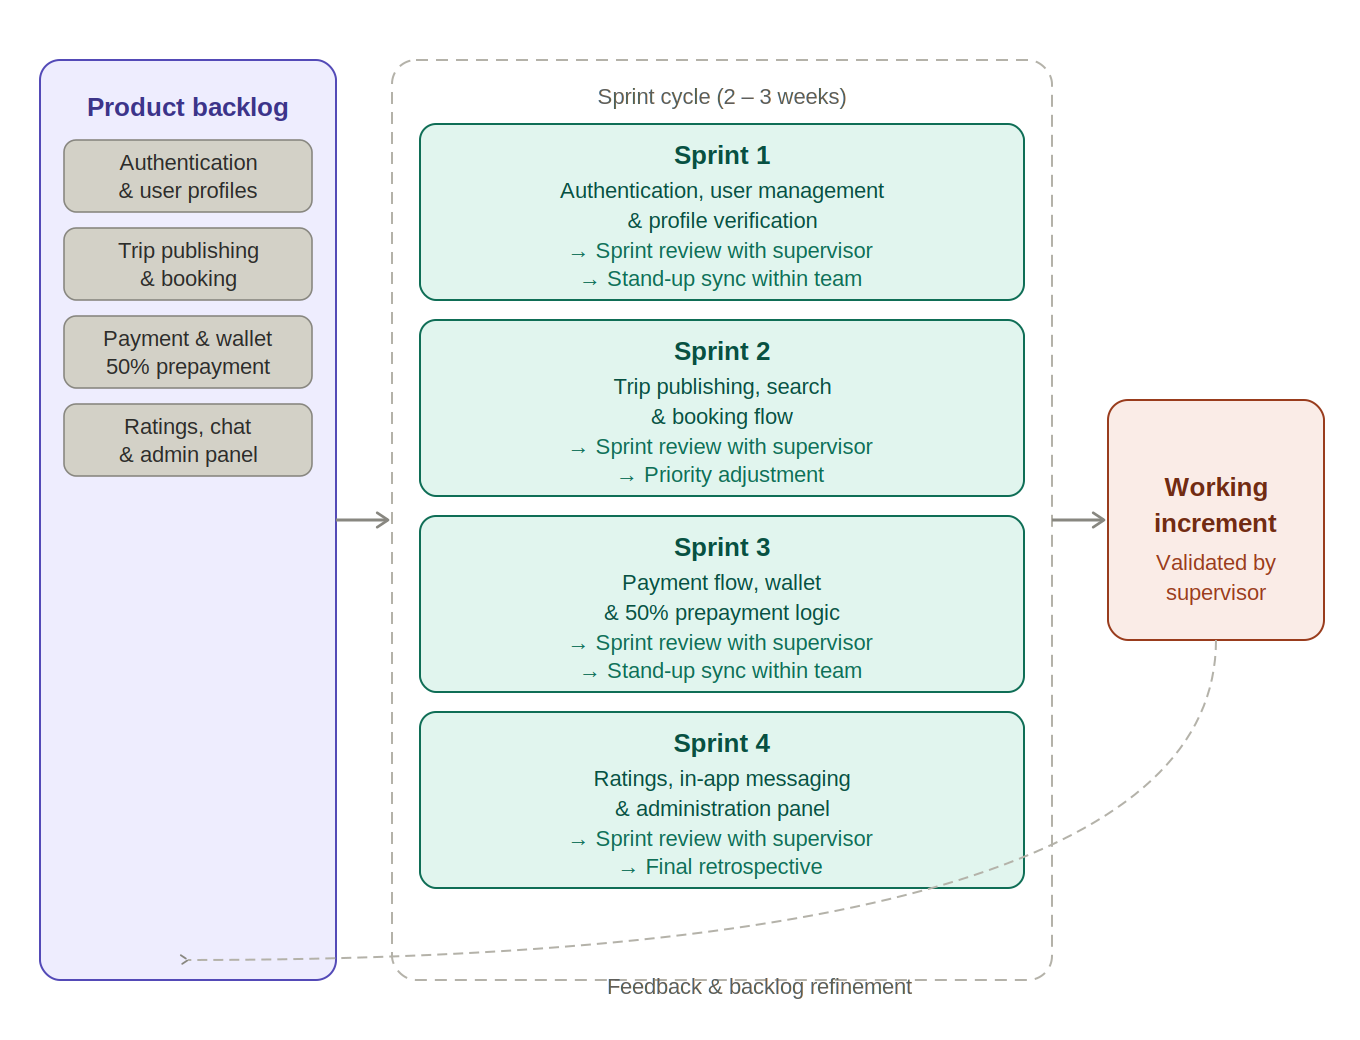
\includegraphics[width=0.9\textwidth]{forsadrive_scrum.png}
    \caption{Overview of the Scrum framework}
    \label{fig:scrum_framework}
\end{figure}

\subsection{Application to ForsaDrive}

In the context of this internship, Scrum was applied in a simplified form adapted to a two-student team. The work was organized into four functional sprints, each of which produced a coherent increment of the platform.

\begin{enumerate}[noitemsep]
    \item \textbf{Sprint 1 — Foundations.} Project setup, authentication, profile management, role management, student verification, driver profile creation, and administrative validation.
    \item \textbf{Sprint 2 — Rides and Bookings.} Ride publishing, search and filtering, single and group bookings, and management of booking requests.
    \item \textbf{Sprint 3 — Payments and Intelligence.} Wallet, fifty-percent prepayment, student discount calculation, ride boosting, driver analytics, and recommendation logic.
    \item \textbf{Sprint 4 — Community and Finalization.} In-app messaging, ratings, complaint handling, social feed, HelpDesk, multilingual support, testing, and deployment.
\end{enumerate}

Short stand-up meetings were held inside the team to coordinate the day-to-day work, and weekly reviews were organized with the supervising engineer to validate progress and adjust priorities. This rhythm proved well suited to a project of this size, since it kept the team focused on a small set of features at a time while preserving the flexibility needed to absorb changes coming from the reviews.


\section{Identification of Actors}

In the UML sense, an actor is any entity, human or automated, that interacts with the system. Four human actors and one automated actor were identified for ForsaDrive.

\begin{description}[noitemsep]
    \item[Guest.] An unauthenticated visitor who can browse the public landing page, consult general information about the platform, and start the registration process.
    \item[Passenger.] A registered user looking for a trip. A passenger can search for available rides, book seats, pay the prepayment, communicate with the driver, and rate the trip after its completion.
    \item[Driver.] A registered user who offers trips. A driver can create, modify, or cancel rides, accept or decline booking requests, and receive payments through the platform.
    \item[Administrator.] The operator of the platform. The administrator is responsible for verifying user identities, validating student documents, moderating reported content, handling disputes, and supervising the overall activity of the platform.
    \item[System.] An automated actor that triggers operations such as the calculation of the student discount, the dispatch of notifications, and the recomputation of the reliability score after each completed trip.
\end{description}

The role of \textit{Student} is not modeled as a separate actor but as a status attached to a passenger account. This status is granted after a successful verification process and gives access to the fifty-percent discount on eligible trips.


\section{Functional Requirements}

Functional requirements describe what the system must do. They are grouped here by actor in order to reflect the structure of the use case diagram presented at the end of the chapter.

\subsection{Requirements for the Guest}

\begin{itemize}[noitemsep]
    \item Browse the public landing page and consult general information about the platform.
    \item Register a new account, choosing between a passenger and a driver role.
    \item Authenticate through email and password.
    \item Recover a forgotten password through a secure procedure.
\end{itemize}

\subsection{Requirements for the Passenger}

\begin{itemize}[noitemsep]
    \item Search for trips by departure city, arrival city, and date.
    \item Filter results by price, departure time, and driver rating.
    \item Consult the full details of a trip, including the profile of the driver.
    \item Reserve one or several seats on a trip.
    \item Pay fifty percent of the amount as a prepayment at the moment of booking.
    \item Benefit from the student discount once the account is verified as such.
    \item Cancel a booking under the cancellation rules defined by the platform.
    \item Rate and review a driver after a completed trip.
    \item Exchange messages with a driver through the in-app chat.
\end{itemize}

\subsection{Requirements for the Driver}

\begin{itemize}[noitemsep]
    \item Publish a new trip with its origin, destination, date, time, price, and number of available seats.
    \item Modify or cancel an existing trip while respecting the rules that protect already booked passengers.
    \item View and manage incoming booking requests.
    \item Access a wallet that summarizes earned, pending, and refunded amounts.
    \item Receive notifications about new bookings and incoming messages.
    \item Rate a passenger after a completed trip.
\end{itemize}

\subsection{Requirements for the Administrator}

\begin{itemize}[noitemsep]
    \item Authenticate through a dedicated administration panel.
    \item Manage user accounts (activation, deactivation, verification).
    \item Review and validate identity documents and student cards.
    \item Moderate reported trips, users, or messages.
    \item Consult global statistics on users, trips, and payments.
\end{itemize}


\section{Non-Functional Requirements}

Non-functional requirements describe the quality attributes that the system must respect. They constrain the design as much as the functional requirements do, since they directly affect the trust that users place in the platform.

\begin{description}[noitemsep]
    \item[Security.] Authentication relies on hashed passwords. Sensitive operations such as payment and account modification require an active and validated session. All exchanges between client and server are protected by HTTPS, and identity documents are stored in a dedicated, access-controlled location.
    \item[Performance.] The system must remain responsive under normal load. Search results, in particular, must be returned within a delay short enough to preserve a fluid user experience.
    \item[Availability.] The platform must remain reachable at all times, except during scheduled maintenance windows announced in advance to the users.
    \item[Usability.] The interfaces are clear and consistent across the web and mobile platforms. A new user must be able to book a trip without external assistance, which requires careful attention to information density, form validation, and feedback messages.
    \item[Portability.] The mobile application runs on recent versions of Android and iOS. The web application is compatible with the major modern browsers.
    \item[Scalability.] The architecture allows new features to be added without rewriting existing modules. This is particularly important for ForsaDrive, since the roadmap includes intelligent services that will be plugged into the existing booking workflow.
    \item[Maintainability.] The source code follows clear conventions and a layered organization, so that a new contributor can become productive within a reasonable amount of time.
\end{description}


\section{Global Use Case Diagram}

The global use case diagram synthesizes the main interactions between the actors and the system. It provides the first complete view of the functional coverage of ForsaDrive and serves as the entry point for the conception phase of the next chapter.

\begin{figure}[H]
    \centering
    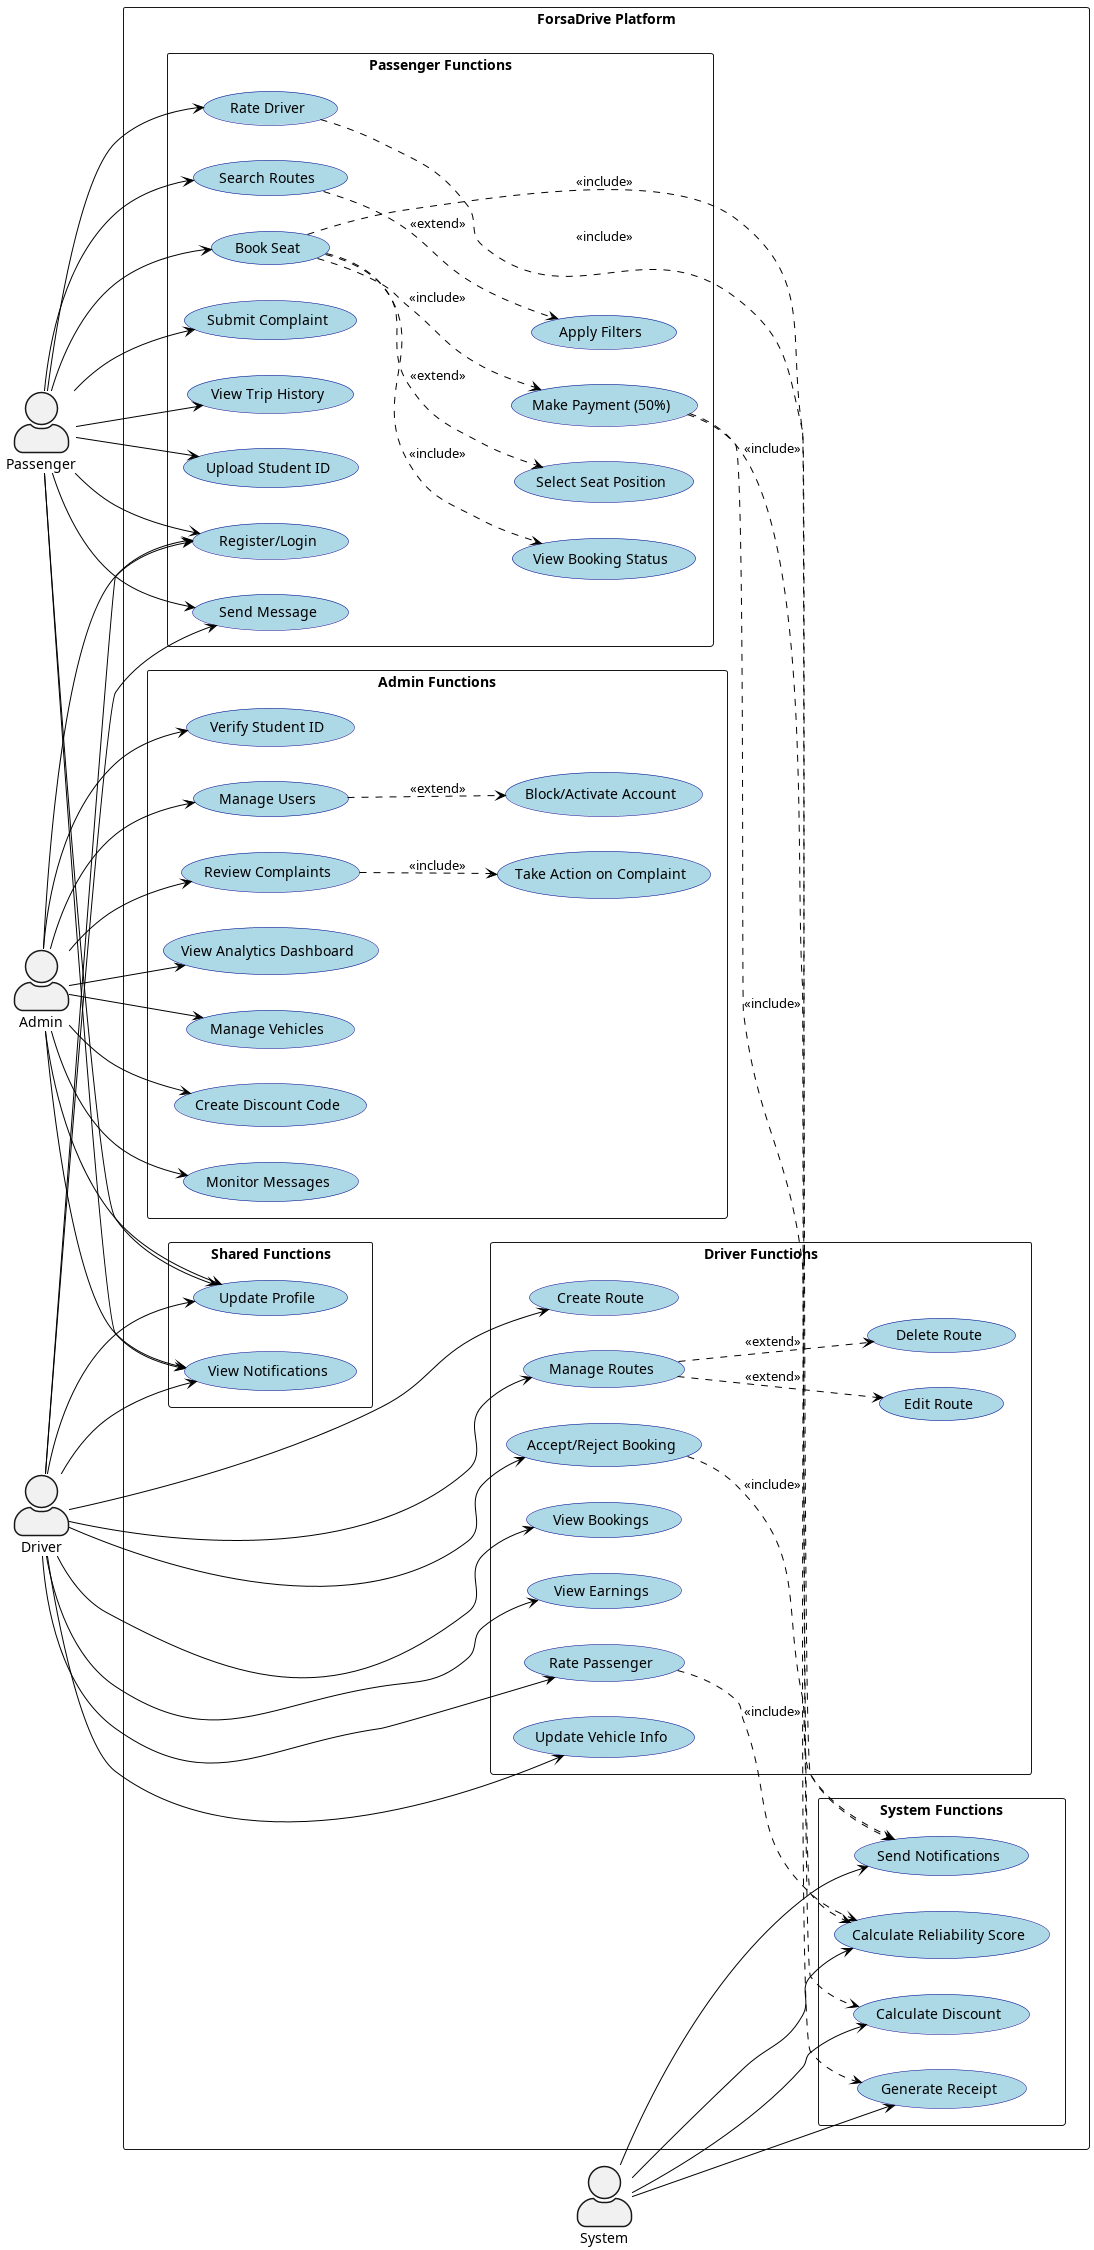
\includegraphics[width=0.7\textwidth]{ForsaDrive_UseCase.png}
    \caption{Global use case diagram of ForsaDrive}
    \label{fig:global_use_case}
\end{figure}


\section*{Conclusion}

This chapter defined the functional scope of ForsaDrive. The comparative study of existing solutions confirmed the absence of a carpooling platform genuinely adapted to the Tunisian context and clarified the gap that the project aims to fill. The presentation of the Scrum methodology and its concrete application to a four-sprint plan introduced the rhythm under which the work was carried out. The identification of the actors and the listing of the functional and non-functional requirements then translated the high-level objectives of the project into a precise specification, which is summarized in the global use case diagram. The next chapter takes this specification as input and produces a detailed conception of the platform, covering its architecture, the dynamic behavior of its most representative scenarios, and the structure of its data.
        \clearpage

        %=============================================================================
%  CHAPTER 3 — SPRINT 0: ARCHITECTURE AND GENERAL CONCEPTION
%=============================================================================
\chapter{Sprint 0: Architecture and General Conception}

\clearpage
\section*{Introduction}

In a Scrum project, Sprint 0 does not yet deliver a usable feature. Its role is to put in place everything the team will need before the first functional sprint can be planned: the technical architecture, the shared vocabulary, the general data model, and the recurring conventions that the rest of the iterations will reuse. We treated Sprint 0 of ForsaDrive in the same spirit. Over roughly the first two weeks of the internship, the focus was less on producing screens and more on settling the questions that, if left open, would have slowed down every later sprint. This chapter reports on that work. It describes the architecture that was retained for the platform, the way the most representative use cases of the global diagram were refined, and the structural backbone of the application through its class diagram and its relational schema.

\section{Sprint 0 Backlog and Objectives}

Before describing the deliverables, it is useful to recall the perimeter of Sprint~0. The product backlog at this point did not contain user stories in the strict sense, since no end user feature was yet targeted. It contained the technical and methodological items that the team needed to validate before starting Sprint~1. Table~\ref{tab:sprint0_backlog} gives an extract of what was placed in this preliminary backlog.

\begin{table}[H]
\centering
\caption{Sprint 0 backlog — preparatory items}
\label{tab:sprint0_backlog}
\begin{tabular}{|p{3.5cm}|p{9cm}|c|}
\hline
\textbf{Item} & \textbf{Description} & \textbf{Estimate (h)} \\
\hline
Architecture choice & Decide on the deployment topology, the API style, and the boundary with external services. & 6 \\
\hline
Stack validation & Confirm that PHP, SQLite, and Flutter can share the same database file in WAL mode. & 8 \\
\hline
Repository layout & Set up the monorepo with the \texttt{web/}, \texttt{mobile/}, and shared backend folders. & 4 \\
\hline
Use case refinement & Detail the four most sensitive use cases identified in chapter~2. & 10 \\
\hline
Class diagram & Produce the structural model covering the core and the secondary entities. & 12 \\
\hline
Relational schema & Translate the class diagram into a normalized schema, with constraints and indexes. & 8 \\
\hline
Coding conventions & Agree on naming, error format, and commit message style. & 3 \\
\hline
\end{tabular}
\end{table}

The estimates are deliberately rough. As is often the case during Sprint~0, several items overlapped: the architecture choice and the stack validation, for example, could not be separated cleanly because validating the stack \textit{was} part of choosing the architecture. The team kept track of the work through a simple Trello board with three columns and updated it at the end of each working day.

\section{General Architecture}

\subsection{Client--Server Topology}

ForsaDrive is organized around a classic client--server topology. A unified REST API is exposed by a backend server and is consumed by two distinct clients: a web application targeted at administrators and at desktop users, and a mobile application that covers the daily usage of drivers and passengers. This separation has two main benefits. It allows the two interfaces to evolve at their own pace, as long as the API contract remains stable, and it avoids duplicating the business logic on the client side, where it would be both harder to maintain and easier to bypass. External services such as the payment gateway, the notification service, and the file storage that hosts student identity documents are reached exclusively through the backend, so that no sensitive credential is ever exposed on a client device.

\begin{figure}[H]
    \centering
    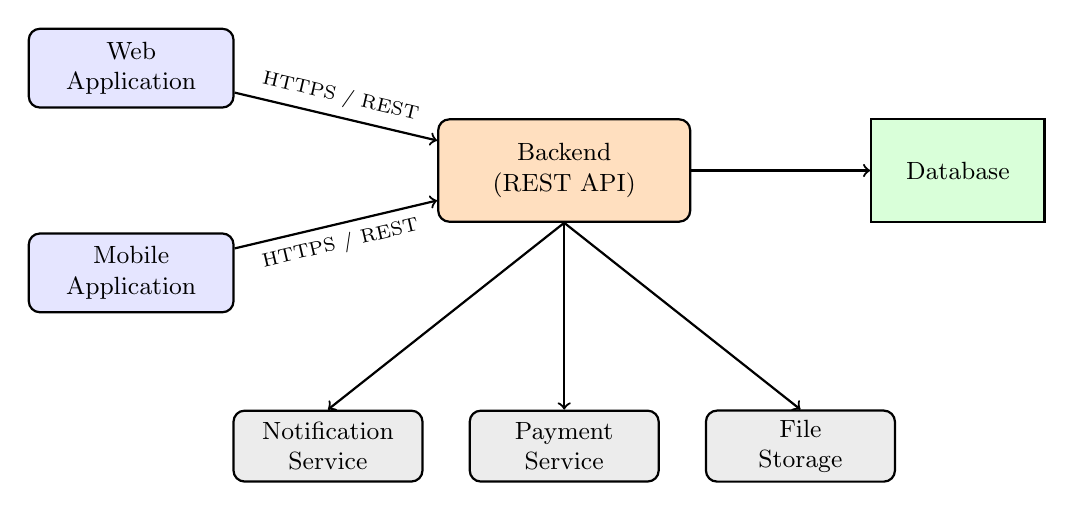
\begin{tikzpicture}[
        every node/.style={font=\small},
        client/.style={draw, rounded corners, minimum width=2.6cm, minimum height=1cm, fill=blue!10, thick, align=center},
        server/.style={draw, rounded corners, minimum width=3.2cm, minimum height=1.3cm, fill=orange!25, thick, align=center},
        db/.style={draw, minimum width=2.2cm, minimum height=1.3cm, fill=green!15, thick, align=center},
        ext/.style={draw, rounded corners, minimum width=2.4cm, minimum height=0.9cm, fill=gray!15, thick, align=center}
    ]
        \node[client] (web)    at (0,  1.3) {Web\\ Application};
        \node[client] (mobile) at (0, -1.3) {Mobile\\ Application};
        \node[server] (api) at (5.5, 0) {Backend\\ (REST API)};
        \node[db] (db) at (10.5, 0) {Database};
        \node[ext] (notif) at (2.5, -3.5) {Notification\\ Service};
        \node[ext] (pay)   at (5.5, -3.5) {Payment\\ Service};
        \node[ext] (store) at (8.5, -3.5) {File\\ Storage};
        \draw[->, thick] (web)        -- (api) node[midway, above, sloped] {\scriptsize HTTPS / REST};
        \draw[->, thick] (mobile)     -- (api) node[midway, below, sloped] {\scriptsize HTTPS / REST};
        \draw[->, thick] (api)        -- (db);
        \draw[->, thick] (api.south)  -- (notif.north);
        \draw[->, thick] (api.south)  -- (pay.north);
        \draw[->, thick] (api.south)  -- (store.north);
    \end{tikzpicture}
    \caption{Client--server architecture of ForsaDrive}
    \label{fig:client_server_architecture}
\end{figure}

\subsection{Three-Tier Internal Organization}

Internally, the backend follows a three-tier organization that separates presentation, business logic, and data persistence. This decomposition reflects a deliberate effort to isolate the parts of the system that change at different rhythms: the presentation tier evolves with the user interface, the application tier with the business rules, and the data tier with the persistence model.

\begin{description}[noitemsep]
    \item[Presentation tier.] Composed of the web and mobile applications, this layer is responsible for user interaction, form validation on the client side, and rendering. It never accesses the database directly and only communicates with the application tier through the REST API.
    \item[Application tier.] Contains the business rules of ForsaDrive: route publication, booking logic, prepayment computation, application of the student discount, ride lifecycle, ratings and reliability scoring, and complaint handling. It is exposed through a REST API secured by bearer tokens.
    \item[Data tier.] Stores persistent information such as users, routes, bookings, payments, ratings, and messages. It is accessed exclusively through the application tier, which guarantees the integrity of the business rules at all times.
\end{description}

\begin{figure}[H]
    \centering
    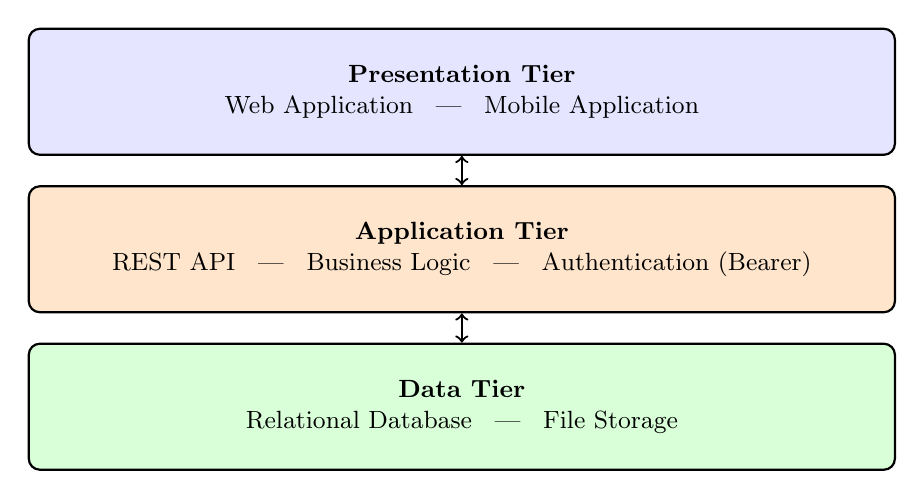
\begin{tikzpicture}[
        every node/.style={font=\small, align=center},
        tier/.style={draw, rounded corners, minimum width=11cm, minimum height=1.6cm, thick}
    ]
        \node[tier, fill=blue!10]   (pres) at (0, 4) {\textbf{Presentation Tier}\\ Web Application \;\;|\;\; Mobile Application};
        \node[tier, fill=orange!20] (app)  at (0, 2) {\textbf{Application Tier}\\ REST API \;\;|\;\; Business Logic \;\;|\;\; Authentication (Bearer)};
        \node[tier, fill=green!15]  (data) at (0, 0) {\textbf{Data Tier}\\ Relational Database \;\;|\;\; File Storage};
        \draw[<->, thick] (pres) -- (app);
        \draw[<->, thick] (app)  -- (data);
    \end{tikzpicture}
    \caption{Three-tier organization of the platform}
    \label{fig:three_tier_architecture}
\end{figure}

\subsection{External Services}

In addition to its own three tiers, the backend interacts with three external building blocks. The \textbf{payment service} is responsible for the fifty-percent prepayment that confirms a booking. In the first version of ForsaDrive this service is simulated through a local wallet, since no Tunisian payment gateway could be integrated within the duration of the internship; the architecture, however, is designed so that this layer can be replaced by a real provider such as Konnect or Paymee without changing the booking logic itself. The \textbf{notification service} delivers booking, payment, and message alerts to drivers and passengers, both through push notifications on the mobile application and through email when relevant. Finally, a dedicated \textbf{file storage} keeps student identity documents and profile pictures separately from the relational database, which keeps the SQLite file small and allows documents to be served through short-lived signed URLs that protect them from unauthorized access.

\subsection{Security Mechanisms}

Authentication relies on randomly generated bearer tokens delivered after a successful login. Every protected endpoint validates the token, extracts the user identity from the \texttt{api\_tokens} table, and checks the associated role before executing the requested operation. Passwords are hashed with \texttt{password\_hash} (bcrypt) and are never stored or transmitted in clear. All communications go through HTTPS in production, and sensitive operations such as payment, account suspension, or student verification are logged on the server side for audit purposes. Identity documents stored in the file service are accessible only to authenticated administrators, through signed URLs that expire after a short delay. Together these mechanisms reduce the attack surface of the platform and align its handling of personal data with the expectations of users entrusting their identity documents to the system.

\section{Refinement of the Main Use Cases}

The global use case diagram of ForsaDrive, already presented in chapter~2, regroups the functionalities of the platform around four actors -- the \textit{Passenger}, the \textit{Driver}, the \textit{Admin}, and the \textit{System}. The latter is responsible for automated operations such as discount calculation, reliability scoring, and notification dispatching. Each actor is restricted to a coherent set of use cases, and a few of them are connected through \texttt{<<include>>} or \texttt{<<extend>>} relationships when an operation must trigger an automated step or when a behavior is optional.

The textual refinement of the four most representative use cases is given below. These four were selected because they cut across the largest number of components and therefore drove the deepest design decisions of the project. The remaining use cases follow a similar pattern and are described, sprint by sprint, in chapters~4 and~5.

\subsection{Use Case: Publish a Route}

\textbf{Actor:} Driver.\\
\textbf{Precondition:} The driver is authenticated, the account is active, and a vehicle has been registered on the profile.\\
\textbf{Main scenario:}
\begin{enumerate}[noitemsep]
    \item The driver selects the action of creating a new route.
    \item The system displays the route creation form.
    \item The driver fills in the origin, the destination, the departure date and time, the price per seat, and the number of available seats.
    \item The driver confirms the creation.
    \item The system validates the data, persists the route with the status \textit{ACTIVE}, and notifies the passengers whose saved searches match the new offer.
\end{enumerate}
\textbf{Alternative scenarios:}
\begin{itemize}[noitemsep]
    \item If a mandatory field is missing or invalid, the system displays an error message and the route is not created.
    \item If the driver account is suspended, the system rejects the request with an explanatory message.
    \item If no vehicle is registered yet, the driver is redirected to the vehicle registration page.
\end{itemize}

\subsection{Use Case: Book a Ride}

\textbf{Actor:} Passenger.\\
\textbf{Precondition:} The passenger is authenticated and at least one seat is available on the selected route.\\
\textbf{Main scenario:}
\begin{enumerate}[noitemsep]
    \item The passenger searches for routes by entering origin, destination, and date.
    \item The system returns the matching routes and applies the student discount on the displayed price if the passenger is a verified student.
    \item The passenger opens the details of a route and selects the number of seats.
    \item The system computes the total amount and the fifty-percent prepayment.
    \item The passenger confirms the booking and the prepayment.
    \item The system processes the prepayment, registers the booking with the status \textit{PENDING}, and notifies the driver.
\end{enumerate}
\textbf{Alternative scenarios:}
\begin{itemize}[noitemsep]
    \item If the prepayment fails, the booking is not created and the passenger is invited to retry or to cancel.
    \item If the seat becomes unavailable between the selection and the confirmation, the booking is rejected and the passenger is informed.
    \item If the driver later refuses the booking, the prepayment is automatically refunded.
\end{itemize}

\subsection{Use Case: Verify Student Status via Email OTP}

\textbf{Actor:} Passenger (Student).\\
\textbf{Precondition:} The passenger is authenticated and possesses a valid university email address whose domain is listed in the platform's recognized domain table.\\
\textbf{Main scenario:}
\begin{enumerate}[noitemsep]
    \item The passenger navigates to the student verification screen and enters a university email address.
    \item The system checks the email domain against the \textit{student\_domains} table maintained by the administrator.
    \item If the domain is recognized, the system generates a six-digit OTP, stores it with a ten-minute expiry, and dispatches it by email to the provided address.
    \item The passenger enters the received code on the verification screen.
    \item The system validates the code, marks the account as \textit{is\_student = true}, and records the verification event in the audit log.
    \item The fifty-percent student discount is automatically applied to all future bookings from this account.
\end{enumerate}
\textbf{Alternative scenarios:}
\begin{itemize}[noitemsep]
    \item If the domain is not in the recognized list, the system rejects the request and shows the list of accepted university domains.
    \item If the code has expired, the student is invited to request a new one.
    \item After five consecutive incorrect attempts the current code is invalidated and the student must request a new one.
\end{itemize}

\subsection{Use Case: Driver Application and Admin Approval}

\textbf{Actors:} Passenger (applicant) and Administrator.\\
\textbf{Precondition:} The applicant is authenticated as a passenger.\\
\textbf{Main scenario:}
\begin{enumerate}[noitemsep]
    \item The applicant opens the \textit{Become a Driver} form and fills in personal details, license number, and vehicle information.
    \item The system stores the application with the status \textit{PENDING} and notifies the administrator.
    \item The administrator reviews the application in the dedicated tab of the admin panel.
    \item Upon approval, the system creates the driver profile, the vehicle record, switches the user role to \textit{DRIVER}, and notifies the applicant.
\end{enumerate}
\textbf{Alternative scenario:}
\begin{itemize}[noitemsep]
    \item Upon rejection, the system stores the rejection reason on the application and notifies the applicant. The user remains a passenger.
\end{itemize}

\section{Class Diagram}

The class diagram describes the structural backbone of the application. Given the breadth of the platform, the diagram regroups around twenty classes that cover not only the core booking entities but also the secondary features that have been identified as relevant for a Tunisian carpooling platform: student verification, complaints, ratings, route boosting, social feed, and analytics. The full diagram is shown in Figure~\ref{fig:class_diagram}.

\begin{figure}[H]
    \centering
    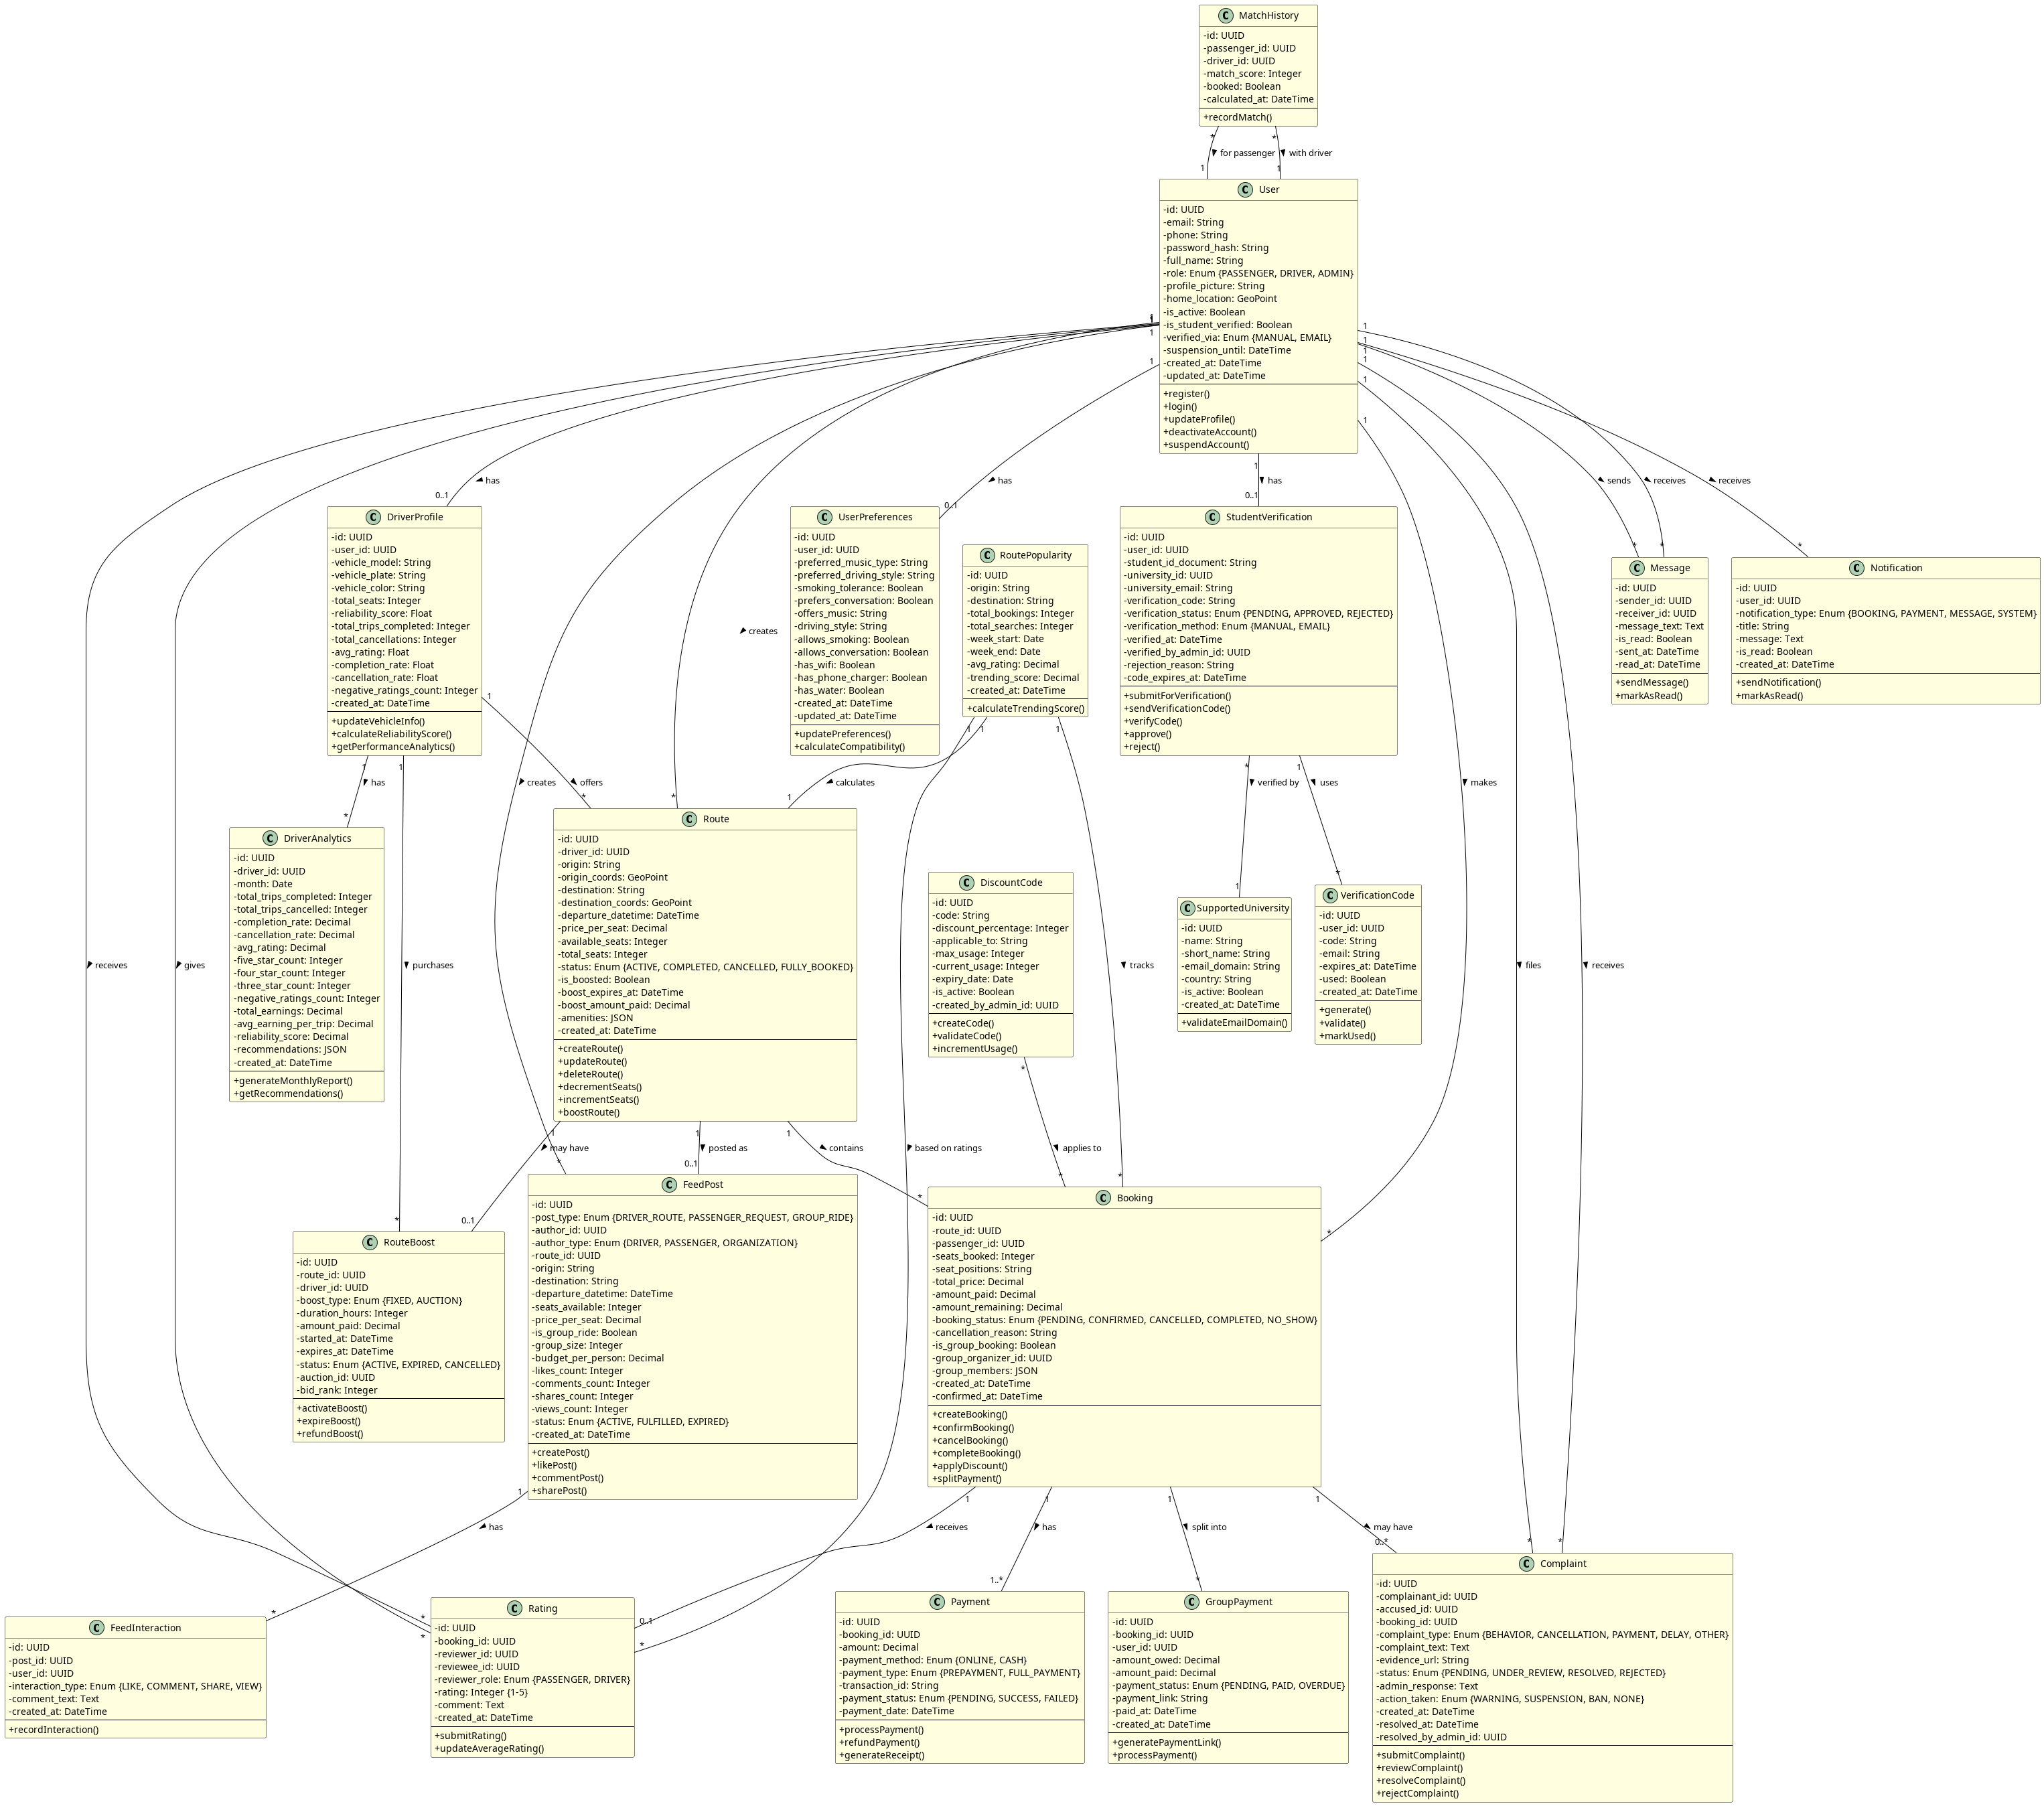
\includegraphics[width=\textwidth, height=0.9\textheight, keepaspectratio]{forsadrive_class_diagram.png}
    \caption{Class diagram of ForsaDrive}
    \label{fig:class_diagram}
\end{figure}

For readability, the main classes are organized into five logical groups.

\paragraph{Users and profiles.} The class \textit{User} represents any registered account and centralizes the credentials, the personal information, the verification status, and the role (\textit{PASSENGER}, \textit{DRIVER}, or \textit{ADMIN}). It is enriched by \textit{DriverProfile}, which holds the vehicle information and the reliability indicators of a driver, and by \textit{UserPreferences}, which describes the preferred travel conditions of a user (music, conversation, smoking tolerance, on-board amenities).

\paragraph{Trips and bookings.} The class \textit{Route} represents a ride offered by a driver, with its origin, its destination, its date, its price, and its available seats. \textit{Booking} represents a reservation made by a passenger on a route and stores the booked seats, the total amount, the prepayment, and the booking status. The optional class \textit{GroupPayment} models the splitting of a booking among several passengers traveling together.

\paragraph{Payments and ratings.} The class \textit{Payment} represents the financial operations linked to a booking, whether it is the prepayment or the final settlement. \textit{Rating} represents the feedback left by a user after a completed trip and feeds back into the average score and the reliability indicators stored on \textit{DriverProfile}.

\paragraph{Verification and discounts.} The class \textit{StudentVerification} stores a verification request, with the uploaded document, the declared university, and the decision of the administrator. It is supported by \textit{SupportedUniversity}, which lists the institutions whose email domains are recognized by the platform, and by \textit{VerificationCode}, which manages email verification codes. The class \textit{DiscountCode} models promotional codes that can be applied at booking time.

\paragraph{Communication and moderation.} The classes \textit{Message} and \textit{Notification} carry the conversations between users and the alerts emitted by the system. \textit{Complaint} allows a user to report a problem after a trip and gives the administrator the means to take action, ranging from a warning to a permanent ban.

Around these core classes, complementary entities such as \textit{DriverAnalytics}, \textit{RoutePopularity}, \textit{MatchHistory}, \textit{RouteBoost}, \textit{FeedPost}, and \textit{FeedInteraction} support the analytical and social dimension of the platform without polluting the central booking workflow.

\section{Database Design}

The class diagram has been translated into a relational model that serves as the schema of the backend database. The translation follows the standard rules: each persistent class becomes a table, each one-to-many association becomes a foreign key, and many-to-many associations are realized through dedicated join tables.

\subsection{Logical Schema}

The logical schema below uses the conventional notation, where primary keys are underlined and foreign keys are marked with the \# symbol. For the sake of readability, only the most representative tables are listed.

\begin{itemize}[noitemsep]
    \item \textbf{User} (\underline{id\_user}, full\_name, email, phone, password\_hash, role, profile\_picture, is\_active, is\_student\_verified, created\_at, updated\_at)
    \item \textbf{DriverProfile} (\underline{id\_driver\_profile}, \#id\_user, vehicle\_model, vehicle\_plate, vehicle\_color, total\_seats, avg\_rating, reliability\_score, completion\_rate, cancellation\_rate, created\_at)
    \item \textbf{UserPreferences} (\underline{id\_preferences}, \#id\_user, preferred\_music\_type, prefers\_conversation, smoking\_tolerance, has\_wifi, has\_phone\_charger)
    \item \textbf{Route} (\underline{id\_route}, \#id\_driver, origin, destination, departure\_datetime, price\_per\_seat, total\_seats, available\_seats, status, is\_boosted, created\_at)
    \item \textbf{Booking} (\underline{id\_booking}, \#id\_route, \#id\_passenger, seats\_booked, seat\_positions, total\_price, amount\_paid, amount\_remaining, booking\_status, created\_at, confirmed\_at)
    \item \textbf{Payment} (\underline{id\_payment}, \#id\_booking, amount, payment\_method, payment\_type, transaction\_id, payment\_status, payment\_date)
    \item \textbf{Rating} (\underline{id\_rating}, \#id\_booking, \#id\_reviewer, reviewer\_role, score, comment, created\_at)
    \item \textbf{StudentVerification} (\underline{id\_verification}, \#id\_user, \#id\_university, student\_id\_document, university\_email, verification\_status, verified\_at, \#id\_admin, rejection\_reason)
    \item \textbf{SupportedUniversity} (\underline{id\_university}, name, short\_name, email\_domain, country, is\_active)
    \item \textbf{DiscountCode} (\underline{id\_discount}, code, discount\_percentage, applicable\_to, max\_usage, current\_usage, expiry\_date, is\_active, \#id\_admin)
    \item \textbf{Message} (\underline{id\_message}, \#id\_sender, \#id\_receiver, message\_text, is\_read, sent\_at, read\_at)
    \item \textbf{Notification} (\underline{id\_notification}, \#id\_user, notification\_type, title, message, is\_read, created\_at)
    \item \textbf{Complaint} (\underline{id\_complaint}, \#id\_complainant, \#id\_accused, \#id\_booking, complaint\_type, complaint\_text, evidence\_url, status, action\_taken, created\_at, resolved\_at, \#id\_admin)
\end{itemize}

\subsection{Constraints and Indexing}

A few business rules deserve to be enforced at the database level rather than only in the application code, since this guarantees their consistency even when the data is touched outside the normal application paths. The number of available seats on a route is constrained between zero and the total number of seats. The booking status follows a controlled state machine (\textit{PENDING}, \textit{CONFIRMED}, \textit{CANCELLED}, \textit{COMPLETED}, \textit{NO\_SHOW}) and the corresponding transitions are checked before any update. Indexes are added on the columns that are frequently used for filtering, in particular the origin and the destination of a route, the departure date, and the foreign keys that link bookings to their route and to their passenger. These indexes ensure that the search operation, which is the most frequent action on the platform, remains responsive even as the volume of data grows.

\section{Sprint 0 Review}

At the end of Sprint~0 the team held a review with the supervising engineer. The architectural choices were validated, with one notable adjustment: the initial intention to use a separate authentication library was abandoned in favor of a lighter, in-house token mechanism stored in an \texttt{api\_tokens} table. This kept the backend free of external dependencies that the team did not feel confident maintaining within the available time. The class diagram was approved with minor renaming, and the database schema was retained in its first version. The repository layout, the conventions, and the use case refinements were also accepted. With these foundations in place, the team could enter Sprint~1 with a clear backlog and a stable structure to build on.

\section*{Conclusion}

This chapter described the work of Sprint~0, whose role was to prepare the ground for the functional sprints that follow. The general architecture clarified the boundary between the clients, the backend, and the external services, and identified the security mechanisms that protect the platform. The four most representative use cases were refined in textual form to expose their internal logic and the alternative scenarios. Finally the class diagram and the relational schema laid down the data foundations that every subsequent sprint will reuse. The next chapter opens the first release of the product and reports on Sprint~1 and Sprint~2, which together deliver the foundational features and the core ride-and-booking workflow.

        \clearpage

        %=============================================================================
%  CHAPTER 4 — RELEASE 1: SPRINT 1 (FOUNDATIONS) AND SPRINT 2 (RIDES & BOOKINGS)
%=============================================================================
\chapter{Release 1: Foundations and Core Booking Workflow}

\clearpage
\section*{Introduction}

The first release of ForsaDrive groups the work carried out during Sprint~1 and Sprint~2. The objective of this release was to deliver a usable product as soon as possible, even at the cost of leaving some advanced features for the next release. Sprint~1 focused on the \textit{Foundations}: account creation, authentication, profile management, student verification, the driver application flow, and the administrative validation that controls access to the driver role. Sprint~2 then built the \textit{Rides and Bookings} workflow on top of these foundations: ride publishing, search and filtering, single and group booking, and the management of booking requests by drivers. By the end of the release, a passenger could register, become a verified student, search for a ride, and book a seat with a fifty-percent prepayment, while a driver could publish trips and review the bookings he had received.

This chapter follows the same structure for each sprint: a short presentation of the sprint backlog with the user stories that were planned, a description of the conception artifacts that were produced (sequence and activity diagrams when relevant), the realization of the corresponding screens on the web and on the mobile, and a brief sprint review. Before entering the sprints themselves, the chapter opens with the development environment and the technological choices that were retained for the entire project, since these decisions affect every later sprint and would clutter the discussion if repeated each time.

\section{Development Environment}

\subsection{Hardware Environment}

The platform was developed on two personal workstations used in parallel by the team. Each machine had enough resources to run the development server, the database engine, and the emulators needed during the implementation. The hardware configurations are summarized in Table~\ref{tab:hw_env}.

\begin{table}[H]
\centering
\caption{Hardware environment}
\label{tab:hw_env}
\begin{tabular}{|l|p{9cm}|}
\hline
\textbf{Component}     & \textbf{Configuration} \\
\hline
Processor              & Intel Core i5 / i7 (8th generation or later) \\
\hline
Memory (RAM)           & 8 GB to 16 GB \\
\hline
Storage                & SSD, 256 GB or more \\
\hline
Operating system       & Windows 10/11 and Ubuntu 22.04 \\
\hline
\end{tabular}
\end{table}

\subsection{Software Environment}

The tools used during the project were chosen for their availability, the experience already acquired by the team during the training, and their compatibility with the technological stack. Table~\ref{tab:sw_env} lists the main ones.

\begin{table}[H]
\centering
\caption{Software environment and tooling}
\label{tab:sw_env}
\begin{tabular}{|l|p{9.5cm}|}
\hline
\textbf{Tool} & \textbf{Role in the project} \\
\hline
Visual Studio Code & Main editor for backend and Flutter, with PHP and Dart extensions. \\
\hline
XAMPP / Apache & Local server stack hosting the PHP backend during development. \\
\hline
Android Studio + emulator & Compilation of the Flutter app and execution on virtual devices. \\
\hline
Git and GitHub & Version control and code sharing between the two team members. \\
\hline
Postman & Manual and collection-based testing of the REST API. \\
\hline
DB Browser for SQLite & Inspection and ad-hoc queries on the SQLite database. \\
\hline
PlantUML & Production of the UML diagrams included in the report. \\
\hline
Trello & Lightweight tracking of the sprint backlog and the daily progress. \\
\hline
\end{tabular}
\end{table}

\section{Technologies Used}

The technological choices made at the beginning of the project apply to every sprint. They were driven by three considerations: the constraints of the project, the experience already acquired during the training at the institute, and the standards adopted by the host organization.

\subsection{Frontend Technologies (Web)}

The web interface is built with PHP rendered server-side, combined with HTML5 and Bootstrap~5 for layout and styling. PHP handles routing, session management, and page rendering in a unified server-side model, which avoids the complexity of a separate frontend build step. Bootstrap was chosen for its responsive grid system and for the consistency it brings to a large set of UI components --- forms, modals, tables, navigation bars --- across the many pages of the application. Client-side interactivity is handled with plain JavaScript, without any additional framework. Dynamic behaviors such as form validation, tab switching in the administration panel, and asynchronous calls for real-time feedback are implemented in small, focused scripts.

\subsection{Backend Technologies}

The backend business logic is written in PHP and exposed as a REST API under the \texttt{/api/} route prefix. PHP was selected because the host organization already operates a PHP-based infrastructure, the language is natively supported by XAMPP without any additional runtime, and the team had prior experience with it. The API follows a front-controller pattern: a single \texttt{index.php} entry point parses the URL, dispatches the request to the appropriate handler file, and returns a JSON response. Database access is performed through PDO with parameterized queries, which protects the application against SQL injection.

Authentication relies on randomly generated bearer tokens stored in an \texttt{api\_tokens} table. After a successful login, the server creates a 32-byte hex token with a 30-day expiry and returns it to the client. Every protected endpoint validates the token from the \texttt{Authorization} header and rejects requests that carry an expired or unknown token.

\subsection{Mobile Technology --- Flutter}

Two main options were considered for the mobile application: developing natively for Android and iOS on the one hand, or using a cross-platform framework on the other. Native development would have doubled the effort without providing enough additional value for a ride-sharing use case, so a cross-platform framework was preferred. After a short evaluation against the time budget of the internship and the team's experience, \textbf{Flutter} was selected.

Flutter is an open-source UI toolkit maintained by Google that allows a single Dart codebase to compile into native applications for Android and iOS. Unlike JavaScript-based frameworks that bridge to native components at runtime, Flutter draws its own widgets using the Skia rendering engine, which gives it pixel-perfect consistency across platforms and a very smooth scrolling behavior. The hot-reload feature also significantly accelerated the iterative work during the sprints. Several supporting packages were added on top of the framework: \texttt{go\_router} for declarative navigation, \texttt{provider} for ChangeNotifier-based state management, \texttt{http} for the REST calls, \texttt{shared\_preferences} for the local persistence of the session token and the language, \texttt{flutter\_map} for the interactive map screen, \texttt{firebase\_messaging} for push notifications, and \texttt{flutter\_localizations} for the multilingual interface.

\subsection{Database --- SQLite}

SQLite was selected as the persistent store. It is a file-based, serverless relational database that requires no separate process, which makes it easy to set up, back up, and share between the web and mobile clients through the same shared file. The database runs in WAL (Write-Ahead Logging) mode to support concurrent reads from the mobile application while the web server writes. Indexes are placed on the columns most frequently used for filtering, in particular the origin, the destination, and the departure date of rides. SQLite is acknowledged as a development choice; the limitations of this option for a high-traffic production environment are discussed in the general conclusion.

\section{Sprint 1 --- Foundations}

\subsection{Sprint Goal and Backlog}

Sprint~1 was planned to last roughly three weeks. Its goal was the one most often quoted in Scrum literature: to deliver an environment in which a real user can be created and can authenticate. Without this, no further sprint can be reviewed against actual interactions. The user stories that were placed in the sprint backlog are listed in Table~\ref{tab:sprint1_backlog}. Story points are estimated according to the standard Fibonacci scale.

\begin{table}[H]
\centering
\caption{Sprint 1 backlog}
\label{tab:sprint1_backlog}
\begin{tabular}{|c|p{8.5cm}|c|}
\hline
\textbf{ID} & \textbf{User story} & \textbf{Points} \\
\hline
US1.1 & As a guest, I want to register an account so that I can access the platform. & 5 \\
\hline
US1.2 & As a registered user, I want to log in with my email and password so that I retrieve my session. & 3 \\
\hline
US1.3 & As a user, I want to view and update my profile so that my information stays accurate. & 3 \\
\hline
US1.4 & As a passenger, I want to verify my student status through a university email OTP so that I receive the student discount. & 8 \\
\hline
US1.5 & As a passenger, I want to apply to become a driver by submitting my license and vehicle so that I can publish trips. & 8 \\
\hline
US1.6 & As an admin, I want to review and approve or reject driver applications so that only verified drivers can publish rides. & 5 \\
\hline
US1.7 & As an admin, I want to manage the list of recognized university domains so that the OTP flow remains under control. & 3 \\
\hline
\end{tabular}
\end{table}

\subsection{Detailed Conception}

Two flows from this sprint are sensitive enough to deserve their own sequence diagrams: the self-service student verification, because it involves the email channel and a strict expiration policy, and the driver application with admin approval, because it changes the role of the user and creates side effects on multiple tables.

\begin{figure}[H]
    \centering
    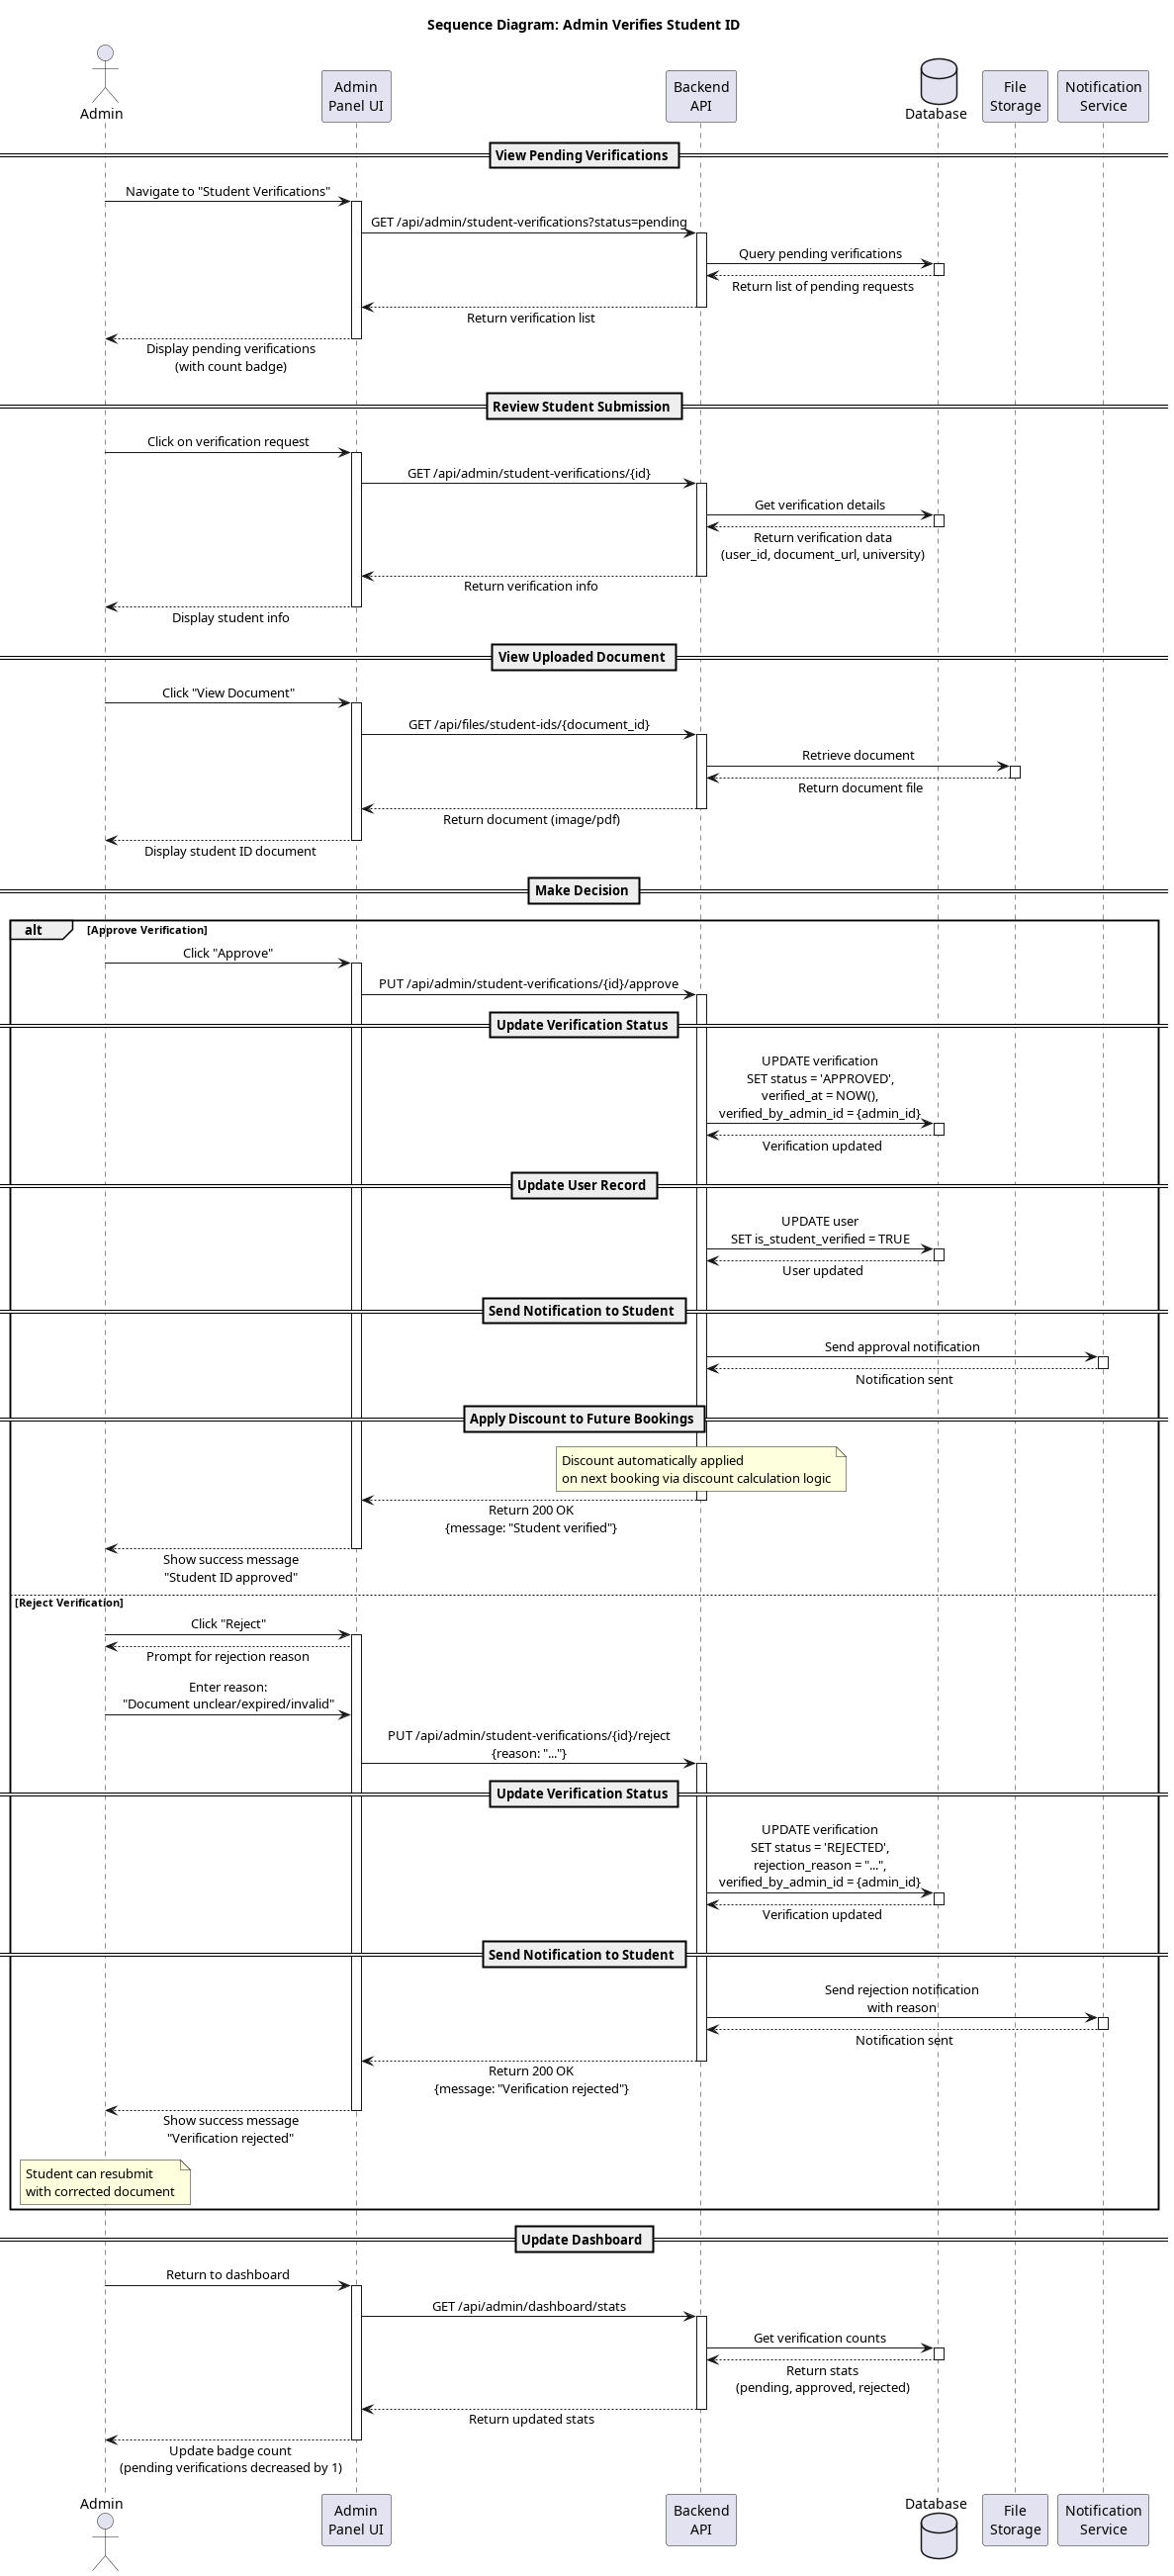
\includegraphics[width=\textwidth, height=0.85\textheight, keepaspectratio]{ForsaDrive_Sequence_VerifyStudent.png}
    \caption{Sequence diagram --- self-service student OTP verification (US1.4)}
    \label{fig:seq_otp_verify}
\end{figure}

The student verification flow opens when the passenger submits a university email address. The backend first checks that the domain is part of the active \texttt{student\_domains} table; if it is not, the user is shown the list of accepted institutions and the request stops there. If the domain is valid, a six-digit code is generated, hashed, and stored together with a ten-minute expiry. The code is then dispatched to the email address. When the user enters the received code, the backend verifies that it has not expired and that no more than five wrong attempts have been made. On success, the \texttt{is\_student\_verified} flag is set on the account and an audit row is written. The student discount is then applied automatically to any subsequent booking.

\begin{figure}[H]
    \centering
    \includegraphics[width=\textwidth, height=0.85\textheight, keepaspectratio]{ForsaDrive_Sequence_DriverApplication.png}
    \caption{Sequence diagram --- driver application and admin approval (US1.5, US1.6)}
    \label{fig:seq_driver_app}
\end{figure}

The driver application flow stores the submitted form with the status \textit{PENDING} and triggers a notification to the administrator. The admin reviews the application in the dedicated tab of the panel. On approval, the backend creates the driver profile, registers the vehicle, switches the role of the user from \textit{PASSENGER} to \textit{DRIVER}, and sends a notification back to the applicant. On rejection, the rejection reason is stored on the application row and the user remains a passenger.

\subsection{Realization}

The screens delivered at the end of Sprint~1 cover the foundations on both clients. The web application opens on a public landing page that introduces the concept and the student discount, with quick access to registration and login (Figure~\ref{fig:web_landing}). The login and registration forms perform validation on the client side for immediate feedback and confirm the inputs on the server (Figure~\ref{fig:web_auth}). The mobile application provides equivalent screens with a real-time student domain detector that highlights the email field in green when the entered address belongs to a recognized university (Figure~\ref{fig:mobile_auth}). The profile screen, common to both clients, gathers the personal information, the verification status with the student badge, and a card showing the status of any pending driver application (Figure~\ref{fig:mobile_profile}).

\begin{figure}[H]
    \centering
    \includegraphics[width=\textwidth]{web_landing.png}
    \caption{Web landing page}
    \label{fig:web_landing}
\end{figure}

\begin{figure}[H]
    \centering
    \includegraphics[width=0.85\textwidth]{web_auth.png}
    \caption{Web authentication interface}
    \label{fig:web_auth}
\end{figure}

\begin{figure}[H]
    \centering
    \includegraphics[width=0.55\textwidth]{mobile_auth.png}
    \caption{Mobile authentication --- login and registration}
    \label{fig:mobile_auth}
\end{figure}

\begin{figure}[H]
    \centering
    \includegraphics[width=0.55\textwidth]{mobile_profile.png}
    \caption{Mobile profile and student badge}
    \label{fig:mobile_profile}
\end{figure}

\subsection{Sprint Review}

The review with the supervising engineer at the end of Sprint~1 confirmed that all user stories of the sprint backlog had been completed. One remark was raised: the very first iteration of the OTP flow allowed a new code to be requested without any cooldown, which would have made the verification endpoint vulnerable to abuse. A thirty-second cooldown between two consecutive requests was added the following day, before opening Sprint~2. The retrospective also highlighted a positive practice that was kept for the rest of the project: writing the form validation rules on the backend first and then mirroring them on the client, rather than the opposite, which avoided the divergence between the two layers that had been observed on a previous course assignment.

\section{Sprint 2 --- Rides and Bookings}

\subsection{Sprint Goal and Backlog}

The goal of Sprint~2 was to deliver the central interaction loop of the platform: a driver publishes a ride, a passenger searches and books it, and the booking is confirmed by a fifty-percent prepayment. The backlog of the sprint is given in Table~\ref{tab:sprint2_backlog}.

\begin{table}[H]
\centering
\caption{Sprint 2 backlog}
\label{tab:sprint2_backlog}
\begin{tabular}{|c|p{8.5cm}|c|}
\hline
\textbf{ID} & \textbf{User story} & \textbf{Points} \\
\hline
US2.1 & As a driver, I want to publish a ride by entering its origin, destination, date, price and seats so that passengers can find it. & 5 \\
\hline
US2.2 & As a driver, I want to modify or cancel a ride that I have published so that I can adjust to last-minute changes. & 3 \\
\hline
US2.3 & As a passenger, I want to search rides by origin, destination and date so that I find the matching offers. & 5 \\
\hline
US2.4 & As a passenger, I want to filter the search results by price, departure time and driver rating so that I narrow down the offers. & 5 \\
\hline
US2.5 & As a passenger, I want to view the full details of a ride and the profile of the driver before booking. & 3 \\
\hline
US2.6 & As a passenger, I want to book one or several seats on a ride with a fifty-percent prepayment so that I confirm the booking. & 8 \\
\hline
US2.7 & As a passenger, I want to book a group seat for friends so that we travel together. & 5 \\
\hline
US2.8 & As a driver, I want to view, accept or reject the incoming booking requests for my rides. & 5 \\
\hline
US2.9 & As a passenger, I want to cancel my booking under the cancellation rules so that I am not stuck with a trip I cannot take. & 3 \\
\hline
\end{tabular}
\end{table}

\subsection{Detailed Conception}

Three diagrams are needed to describe the sprint with sufficient precision: a sequence diagram for the publication of a ride by a driver, a sequence diagram for the booking of a ride by a passenger, and an activity diagram that gives a global view of the booking journey.

\begin{figure}[H]
    \centering
    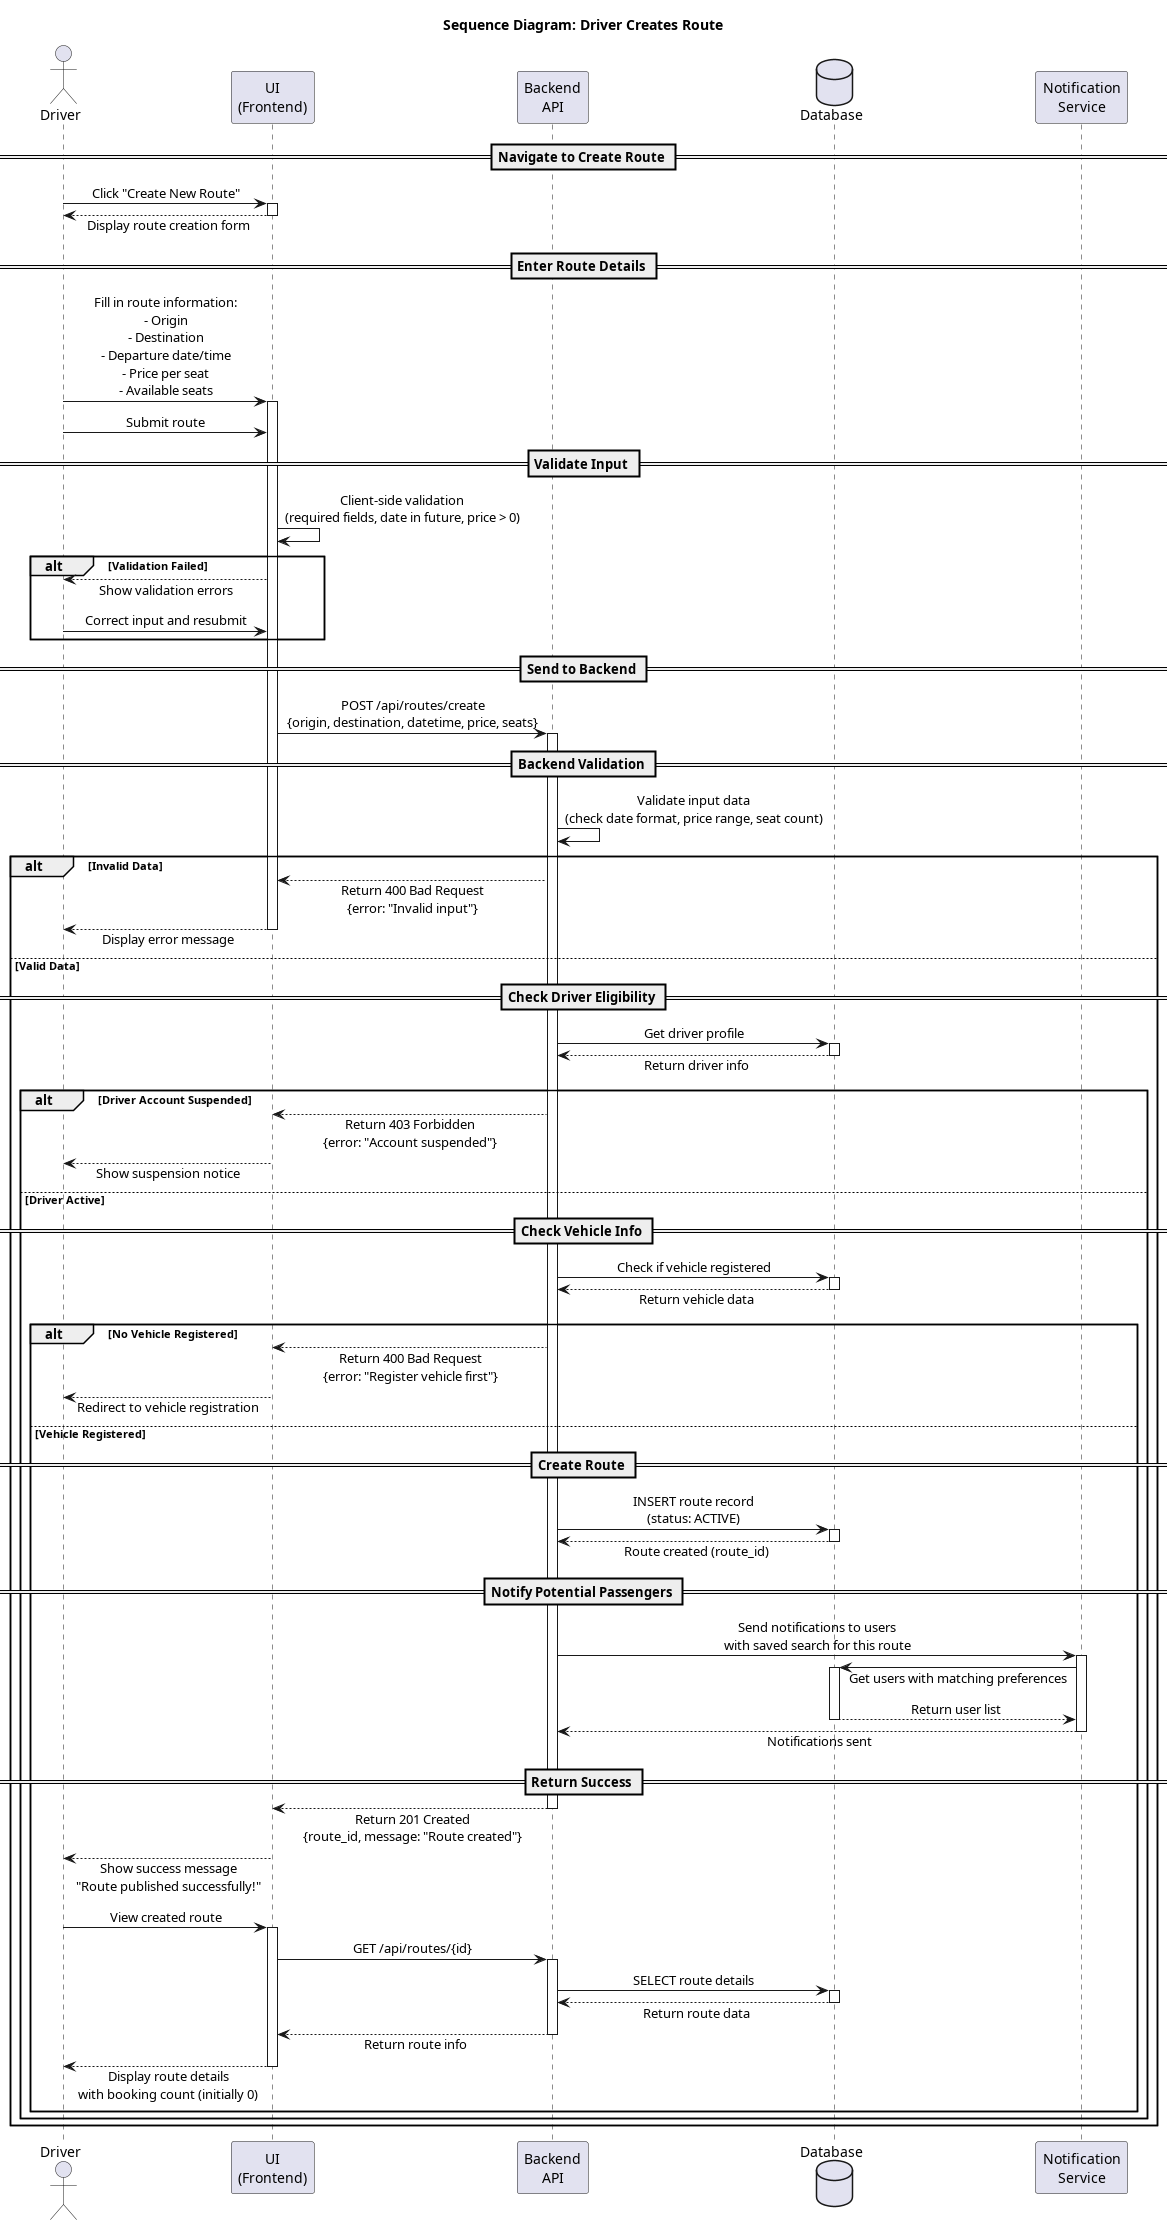
\includegraphics[width=\textwidth, height=0.85\textheight, keepaspectratio]{ForsaDrive_Sequence_CreateRoute.png}
    \caption{Sequence diagram --- driver publishes a route (US2.1)}
    \label{fig:seq_create_route}
\end{figure}

The publication starts with a client-side validation that catches the most common mistakes early. The backend then verifies that the driver account is active, that a vehicle has been registered, and that the requested seat count is consistent with the vehicle. The route is persisted with the status \textit{ACTIVE} and the saved searches that match the new offer trigger a notification.

\begin{figure}[H]
    \centering
    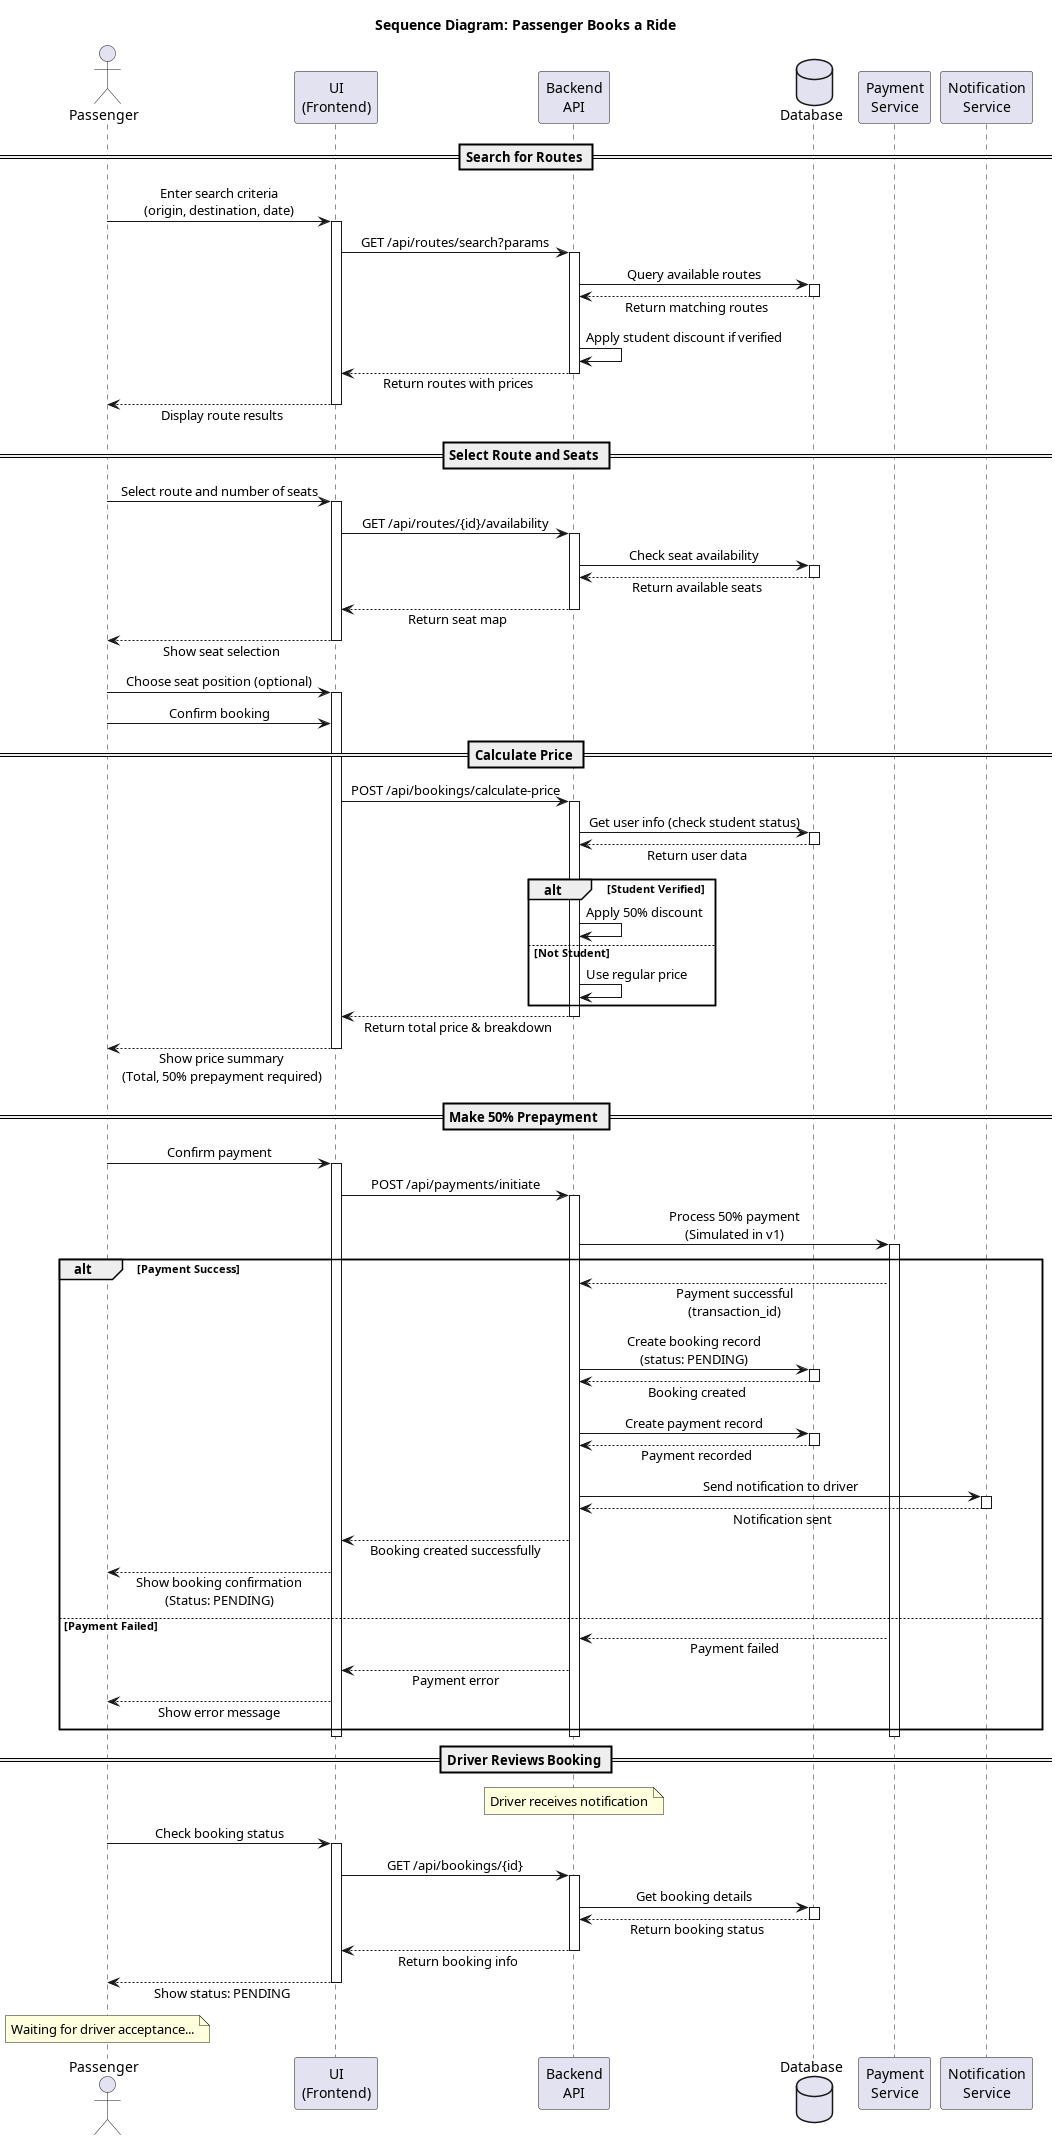
\includegraphics[width=\textwidth, height=0.85\textheight, keepaspectratio]{ForsaDrive_Sequence_BookRide.png}
    \caption{Sequence diagram --- passenger books a ride with prepayment (US2.6)}
    \label{fig:seq_book_ride}
\end{figure}

The booking sequence highlights the interaction between the passenger, the application, the wallet, the notification service, and the database. The student discount is applied at the price computation step, before the prepayment of fifty percent is deducted from the wallet. The booking is only persisted if the deduction succeeds, which guarantees the commitment of the passenger and protects the driver from no-shows.

\begin{figure}[H]
    \centering
    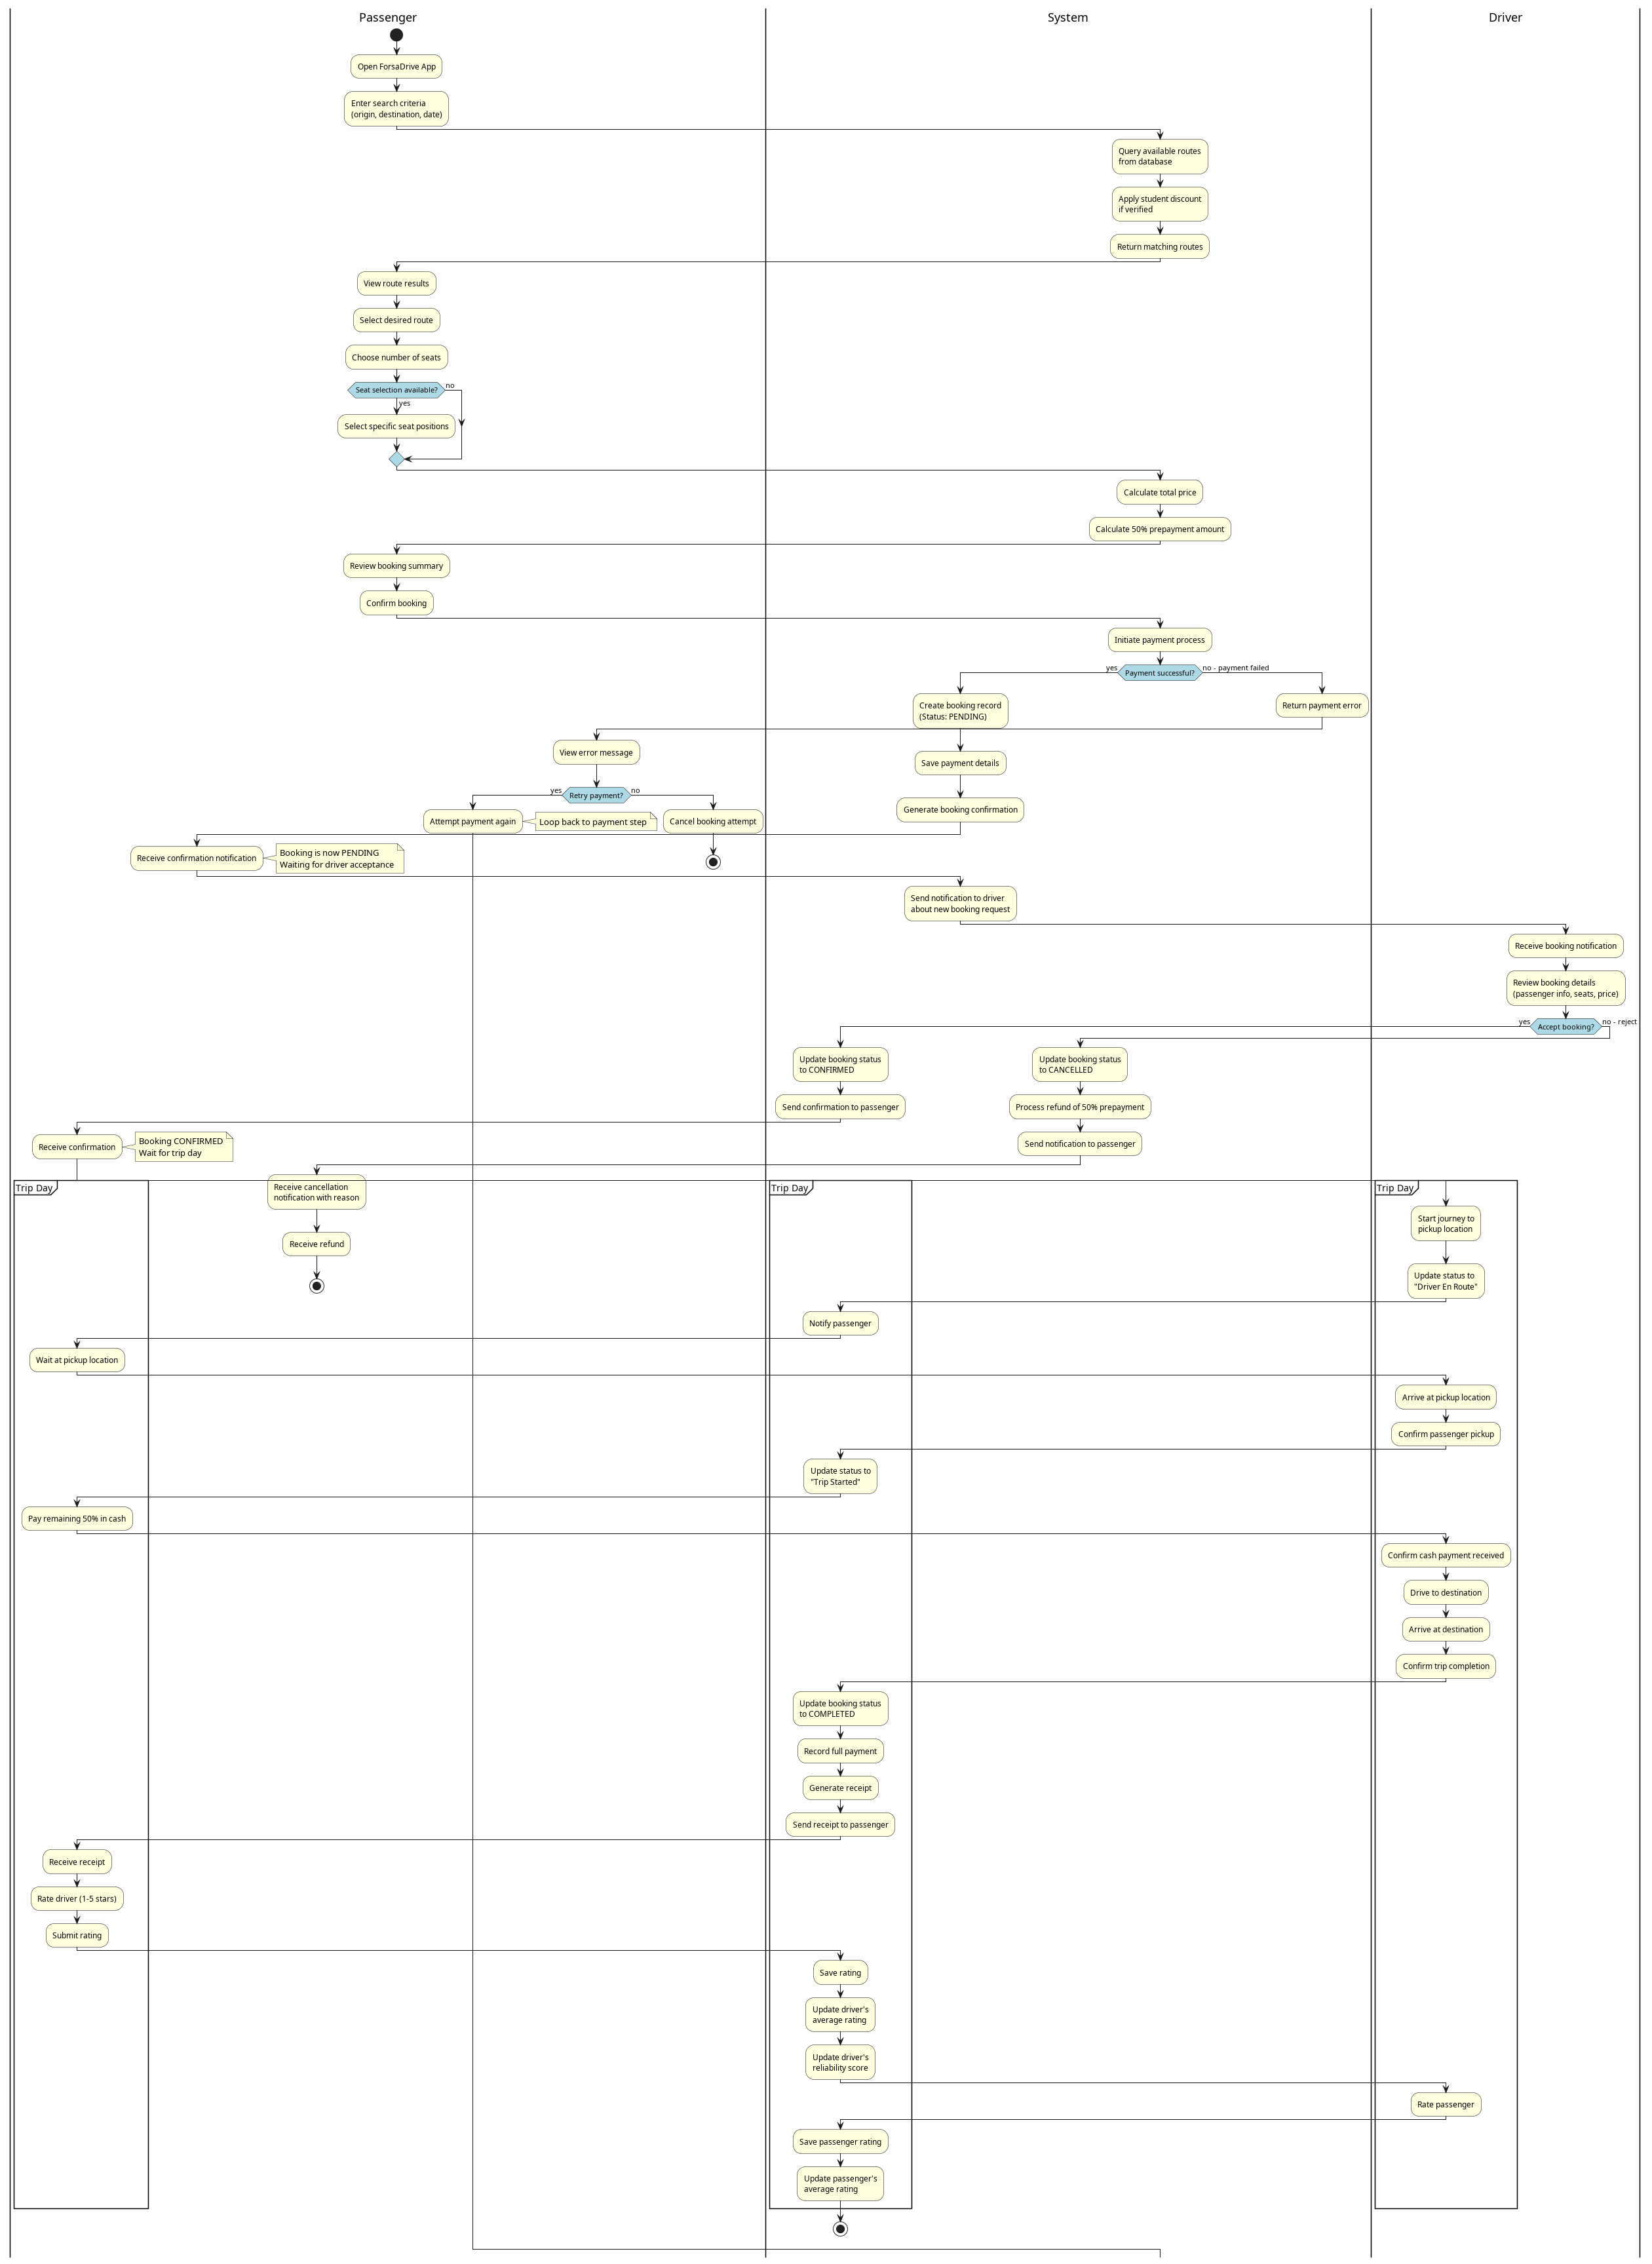
\includegraphics[width=\textwidth, height=0.85\textheight, keepaspectratio]{ForsaDrive_Activity_BookingFlow.png}
    \caption{Activity diagram --- end-to-end booking journey}
    \label{fig:activity_booking_flow}
\end{figure}

The activity diagram complements the sequence diagrams by emphasizing the decision points: the retry of a failed payment, the acceptance or refusal of the booking by the driver, the departure and arrival confirmations, and the cash collection at the end of the trip.

\subsection{Realization}

On the web side, drivers reach the publication form through a dedicated entry in the menu (Figure~\ref{fig:web_publish_trip}). The form requests the mandatory information and shows a preview of how the trip will be displayed to passengers. The search page lets passengers filter trips by origin, destination, date, and preferences, with the results displayed as cards that include the driver's name, the rating, the price, and the remaining seats (Figure~\ref{fig:web_search}). The booking page shows the total amount, the student discount when applicable, and the prepayment, and only confirms the reservation once the prepayment has been registered (Figure~\ref{fig:web_booking}).

\begin{figure}[H]
    \centering
    \includegraphics[width=\textwidth]{web_publish_trip.png}
    \caption{Web --- ride publishing form}
    \label{fig:web_publish_trip}
\end{figure}

\begin{figure}[H]
    \centering
    \includegraphics[width=\textwidth]{web_search.png}
    \caption{Web --- ride search and results}
    \label{fig:web_search}
\end{figure}

\begin{figure}[H]
    \centering
    \includegraphics[width=\textwidth]{web_booking.png}
    \caption{Web --- booking confirmation with prepayment}
    \label{fig:web_booking}
\end{figure}

The mobile application offers the same workflow with a slightly different presentation tailored to the smaller screen. The home screen is centered on a search bar, with a few personalized sections below it that are populated as soon as the user accumulates booking history (Figure~\ref{fig:mobile_home}). The search results screen exposes the same filters as the web side and adds a compatibility score badge on each card, computed from the user's previous bookings and preferences (Figure~\ref{fig:mobile_search}). After selecting a ride, the passenger reaches a detailed view that shows the route on an interactive OpenStreetMap tile, the driver's profile, and the price breakdown including the student discount when applicable. The booking is confirmed after the fifty-percent prepayment is deducted from the wallet (Figure~\ref{fig:mobile_trip_details}).

\begin{figure}[H]
    \centering
    \includegraphics[width=0.55\textwidth]{mobile_home.png}
    \caption{Mobile --- home screen with personalized sections}
    \label{fig:mobile_home}
\end{figure}

\begin{figure}[H]
    \centering
    \includegraphics[width=0.55\textwidth]{mobile_search.png}
    \caption{Mobile --- ride search with filters and match score}
    \label{fig:mobile_search}
\end{figure}

\begin{figure}[H]
    \centering
    \includegraphics[width=0.85\textwidth]{mobile_trip_details.png}
    \caption{Mobile --- trip details with map and booking confirmation}
    \label{fig:mobile_trip_details}
\end{figure}

\subsection{Sprint Review}

The review at the end of Sprint~2 confirmed that the central booking loop was working end to end on both clients. Two adjustments came out of the review and were prioritized for the following sprint: the price filter on the search results was using a fixed maximum of 200~TND, which proved too low for a few long trips, and the group booking flow lacked an explicit confirmation that the passengers traveling together had been informed. The first point was solved by replacing the hard-coded ceiling with a slider whose maximum is computed from the highest ride price in the current result set. The second was deferred to Sprint~4 and ultimately addressed by the in-app chat. The retrospective noted that the time spent on the activity diagram before starting the implementation paid off: the cash collection step, in particular, would otherwise have been forgotten until much later.

\section*{Conclusion}

This chapter reported on the first release of ForsaDrive. Sprint~1 delivered the foundations that every subsequent feature relies on: account creation, authentication, profile management, the self-service student OTP verification, the driver application, and the administrative review that controls access to the driver role. Sprint~2 then built the core interaction loop of the platform, from the publication of a ride to its booking with a fifty-percent prepayment. Together, the two sprints produced an application that already covers the basic carpooling experience and that the team could submit to the supervising engineer for a real demonstration. The next chapter reports on the second release, which adds the wallet, the intelligent features, the community dimension, and the testing and deployment work that closes the project.

        \clearpage

        %=============================================================================
%  CHAPTER 5 — REALIZATION OF THE MOBILE APPLICATION
%=============================================================================
\chapter{Realization of the Mobile Application}

\clearpage
\section*{Introduction}

The mobile application extends the reach of ForsaDrive by making the service available from any smartphone. Because carpooling is, by nature, something users organize on the move --- while leaving a class, waiting for a colleague, or standing at a louage station --- the mobile experience was treated as a first-class citizen and not as an afterthought. This chapter describes the technologies that were used to build it, the features that only make sense on a mobile device, and the main screens delivered at the end of the project. It closes with the testing strategy that was applied to the entire platform.


\section{Mobile Technologies}

\subsection{Choice of a Cross-Platform Framework}

Two main options were considered for the mobile application: developing natively for Android and iOS on the one hand, or using a cross-platform framework on the other. Native development would have doubled the effort without providing enough additional value for a ride-sharing use case, so a cross-platform framework was preferred. After evaluating the alternatives against the time budget of the internship and the team's experience, \textbf{Flutter} was selected.

Flutter is an open-source UI toolkit maintained by Google that allows a single Dart codebase to compile into genuinely native applications for Android, iOS, web, and desktop. Unlike JavaScript-based frameworks that bridge to native components at runtime, Flutter draws its own widgets using the Skia rendering engine, which gives it pixel-perfect consistency across platforms and excellent rendering performance. Its hot-reload feature also significantly accelerated the development cycle during the iterative sprints.

\begin{figure}[H]
    \centering
    \includegraphics[width=0.3\textwidth]{flutter_logo.png}
    \caption{Flutter logo}
    \label{fig:flutter_logo}
\end{figure}

\subsection{Supporting Libraries}

Several packages were added to the Flutter project to cover the specific needs of the application.

\begin{description}[noitemsep]
    \item[go\_router] Manages declarative navigation between screens, deep links, and the bottom tab bar.
    \item[provider] Implements the ChangeNotifier-based state management pattern, used for authentication state, locale, and ride data.
    \item[dio / http] Consumes the REST API exposed by the PHP backend, with the bearer token attached globally through an interceptor.
    \item[shared\_preferences] Persists the session token and the selected language locally on the device so that the user does not have to log in at every launch.
    \item[flutter\_map] Renders interactive OpenStreetMap tiles and draws the route polyline between the origin and the destination of a ride.
    \item[firebase\_messaging] Delivers push notifications for new bookings, confirmations, ride updates, and chat messages, even when the application is in the background.
    \item[flutter\_localizations] Provides the full internationalization infrastructure for French, English, and Arabic, including automatic RTL layout flipping for Arabic.
\end{description}

\section{Mobile-Specific Features}

Beyond mirroring the web experience, the mobile application takes advantage of features that only a phone can provide.

\subsection{Push Notifications}

Push notifications are delivered through Firebase Cloud Messaging. They inform the user of events that require attention: a new booking request for a driver, a booking confirmation or cancellation for a passenger, a ride departure, a new chat message, or an admin action on the account. Notifications are delivered even when the application is in the background, which matches the real usage patterns of the platform.

\subsection{In-App Chat}

The mobile application embeds a real-time messaging interface. Conversations are polled every three seconds to display new messages without requiring a persistent WebSocket connection. The interface shows date dividers, read receipts, and a typing indicator. Passengers and drivers can start a conversation directly from a booking notification without leaving the application.

\subsection{Interactive Map}

Each ride detail screen embeds a \texttt{FlutterMap} widget that geocodes the origin and destination city names using the Nominatim API and draws the driving route between them using the OSRM open routing service. Green and red markers indicate the pickup and drop-off points respectively.

\subsection{Multilingual Interface}

The application supports three languages --- French, English, and Arabic --- with a language picker accessible from the settings screen. Arabic triggers an automatic RTL layout flip through \texttt{GlobalWidgetsLocalizations}, so all padding, alignment, and navigation directions are mirrored without any manual override in the widget code.

\section{Presentation of the Mobile Interfaces}

The following screens illustrate the main paths inside the mobile application. Screens are shown in the order a typical passenger would go through them.

\subsection{Authentication}

The authentication screens cover login, registration, and student email OTP verification. The registration form includes a gender selector, a date-of-birth picker, and a real-time student domain detector that shows a green banner when the entered email belongs to a recognized university domain.

\begin{figure}[H]
    \centering
    \includegraphics[width=0.6\textwidth]{mobile_auth.png}
    \caption{Mobile authentication screens (login and registration)}
    \label{fig:mobile_auth}
\end{figure}

\subsection{Home and Search}

The home screen is centered on a search bar. Below it, three personalized sections are displayed: recommended rides based on the user's booking history (collaborative filtering), trending routes derived from recent bookings, and nearby rides matched to the user's governorate.

\begin{figure}[H]
    \centering
    \includegraphics[width=0.6\textwidth]{mobile_home.png}
    \caption{Home screen with personalized recommendations}
    \label{fig:mobile_home}
\end{figure}

\subsection{Ride Search and Filters}

The search results screen allows passengers to filter rides by price range, minimum driver rating, departure date, number of seats, and on-board amenities (air conditioning, Wi-Fi, music, accessibility). Each ride card displays a compatibility score badge showing how well the ride matches the passenger's profile and history.

\begin{figure}[H]
    \centering
    \includegraphics[width=0.6\textwidth]{mobile_search.png}
    \caption{Ride search results with filters and match score}
    \label{fig:mobile_search}
\end{figure}

\subsection{Trip Details and Booking}

After selecting a ride, the passenger reaches a detailed view that shows the route on an interactive map, the driver's profile and reliability score, and the price breakdown including the student discount when applicable. The booking is confirmed after the fifty-percent prepayment is deducted from the wallet.

\begin{figure}[H]
    \centering
    \includegraphics[width=0.9\textwidth]{mobile_trip_details.png}
    \caption{Trip details with map and booking confirmation}
    \label{fig:mobile_trip_details}
\end{figure}

\subsection{Driver Dashboard}

The driver dashboard is organized into two tabs. The overview tab shows active ride cards with departure and arrival action buttons. The analytics tab presents a reliability score gauge, a six-month revenue trend chart, a rating distribution bar chart, and smart improvement recommendations generated by the backend.

\begin{figure}[H]
    \centering
    \includegraphics[width=0.9\textwidth]{mobile_driver_dashboard.png}
    \caption{Driver dashboard with analytics and reliability score}
    \label{fig:mobile_driver_dashboard}
\end{figure}

\subsection{Wallet}

The wallet screen consolidates the financial activity of the user: current balance, pending amounts, and the history of operations. Drivers also see their earnings grouped by trip.

\begin{figure}[H]
    \centering
    \includegraphics[width=0.6\textwidth]{mobile_wallet.png}
    \caption{Wallet screen}
    \label{fig:mobile_wallet}
\end{figure}

\subsection{Social Feed}

The feed screen lets drivers post ride offers and passengers post travel requests. Posts can be liked, commented on, and used as a direct booking entry point through a quick-booking bottom sheet. Boosted posts appear at the top of the feed and are marked with a ``Boosted'' badge.

\begin{figure}[H]
    \centering
    \includegraphics[width=0.6\textwidth]{mobile_feed.png}
    \caption{Social feed with ride posts and quick booking}
    \label{fig:mobile_feed}
\end{figure}

\subsection{In-App Chat}

The chat screen lists the conversations linked to active trips. Each conversation opens on a messaging view with a bubble layout, date dividers, and read receipts. Drivers can also open a conversation directly from a booking notification.

\begin{figure}[H]
    \centering
    \includegraphics[width=0.6\textwidth]{mobile_chat.png}
    \caption{In-app chat screen}
    \label{fig:mobile_chat}
\end{figure}

\subsection{HelpDesk with AI Bot}

The HelpDesk screen opens a support conversation that is initially handled by a rule-based bot. The bot covers fourteen topic categories and responds instantly to common questions. When the bot cannot resolve the issue, it escalates the conversation to a human support agent and notifies the user.

\begin{figure}[H]
    \centering
    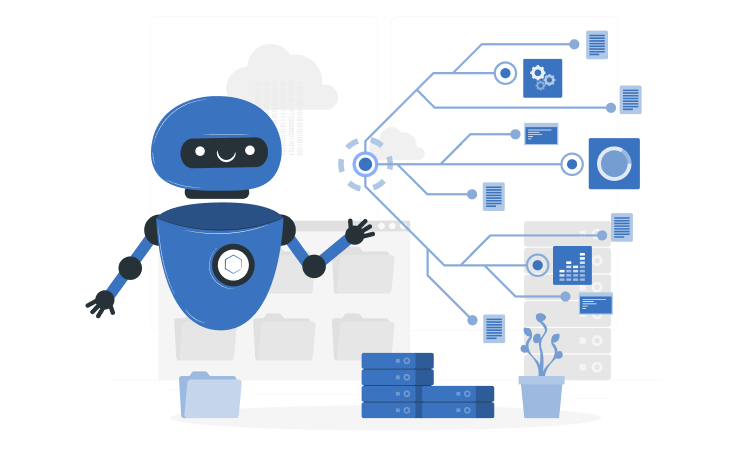
\includegraphics[width=0.6\textwidth]{aibot.png}
    \caption{HelpDesk screen with AI bot and escalation to human agent}
    \label{fig:mobile_helpdesk}
\end{figure}

\subsection{Profile and Settings}

The profile screen gathers the personal information, the verification status including the student badge, the vehicle list, and the language selector. A driver application card shows the status of any pending driver registration request.

\begin{figure}[H]
    \centering
    \includegraphics[width=0.6\textwidth]{mobile_profile.png}
    \caption{Profile and settings screen}
    \label{fig:mobile_profile}
\end{figure}

\section{Testing}

Testing was carried out continuously during the implementation phase, rather than left to a final stage.

\subsection{Unit Testing}

Unit tests were written for the most sensitive business rules of the backend: the computation of the total amount, the application of the student discount, the enforcement of the prepayment percentage, and the validation of user inputs. These tests catch regressions early and serve as a living documentation of the rules.

\subsection{Integration Testing}

Integration tests were performed through Postman collections that replay the main scenarios end to end: registration, login, trip creation, booking, payment, and rating. Each collection was executed after every significant change on the backend.

\subsection{Manual Testing}

Manual tests were conducted on the web application and on the mobile application, including cross-device testing on several Android phones. Feedback from members of the host organization also helped detect usability issues that automated tests cannot catch.

\subsection{Summary of Tests}

\begin{table}[H]
\centering
\caption{Summary of tested scenarios}
\begin{tabular}{|l|c|}
\hline
\textbf{Scenario}                             & \textbf{Result} \\
\hline
Registration and student email OTP verification & Passed \\
\hline
Login and token-based session                 & Passed \\
\hline
Driver application submission and approval    & Passed \\
\hline
Publishing, updating, and cancelling a trip   & Passed \\
\hline
Searching trips with filters and match score  & Passed \\
\hline
Booking with 50\% prepayment                  & Passed \\
\hline
Applying the student discount                 & Passed \\
\hline
Wallet top-up and history                     & Passed \\
\hline
Rating a completed trip                       & Passed \\
\hline
Real-time chat between two users              & Passed \\
\hline
Push notification delivery (FCM)              & Passed \\
\hline
Social feed post, like, comment, quick book   & Passed \\
\hline
Ride boosting with balance deduction          & Passed \\
\hline
Administrator moderation actions (7 tabs)     & Passed \\
\hline
Multilingual switching (FR / EN / AR + RTL)   & Passed \\
\hline
\end{tabular}
\end{table}

\section*{Conclusion}

This chapter closed the realization phase of ForsaDrive by presenting the mobile application and the testing strategy applied to the entire platform. The Flutter client reuses the PHP backend designed in the previous chapters and adds the features that a phone makes possible: push notifications, interactive maps, real-time chat, and a multilingual interface with automatic RTL support. Together with the web application, it delivers the complete ride-sharing experience originally targeted by the project.

        \clearpage

        \chapter*{General Conclusion}
\addcontentsline{toc}{chapter}{General Conclusion}
\markboth{General Conclusion}{}

\par This Final Year Project was carried out within \textbf{ATOMIC IT} as part of the design and development of \textbf{ForsaDrive}, a carpooling platform built specifically for the Tunisian context. The project was delivered as two coordinated applications --- a responsive web platform and a cross-platform mobile application --- both driven by a unified REST API and a shared database.

\par Looking back at the objectives set at the start of the internship, the core requirements have been met. Users can register as passengers or as drivers, search and publish rides, book seats with a fifty-percent prepayment, communicate through in-app chat, and rate each other after a completed trip. Students can verify their status through a university email OTP flow and receive an automatic discount on eligible bookings. Drivers go through a structured application reviewed by an administrator before gaining access to the driver features. The administration panel gives platform operators full control over users, rides, complaints, and organizational accounts.

\par Beyond the initial scope, several features were added progressively as the sprints moved forward and our understanding of the target users deepened. The social feed, the ride boosting system, the AI-assisted helpdesk with bot escalation, the driver analytics dashboard, and the multilingual interface with Arabic RTL support all came out of this ongoing refinement.

\par On the technical side, the project was a genuine learning experience. Coordinating two clients against a single backend required careful API design from the very first sprint. Flutter exposed us to reactive state management and cross-platform rendering in ways that were new to us. Implementing WAL mode on SQLite to allow concurrent reads while the web server writes was one of those concrete problems where solving it gave a much better understanding of database concurrency than any textbook example.

\par The project also has real limitations worth acknowledging. The wallet relies on manual top-ups because no local payment gateway was available for integration within the internship period. SQLite is practical for development but not suited for a high-traffic production environment. The mobile application was tested only on Android, and performance under load was not measured. A forgot-password flow is also missing.

\par These gaps are, in a sense, the roadmap for what comes next. A real deployment would require migrating to PostgreSQL or MySQL, integrating a local payment provider such as Konnect or Paymee, setting up a production server with HTTPS and automated backups, and releasing the Flutter app to the Google Play Store. Two-factor authentication for driver and admin accounts, an offline-first cache for the mobile client, and a password reset email flow would close the remaining security and usability gaps.

\par In a broader sense, this project shows that the technical barriers to a locally adapted carpooling platform are not as high as they might seem. The demand among Tunisian students and commuters is clearly there. What has been missing is a product that fits local payment habits, speaks the right languages, and is designed with an understanding of how trips are actually organized in Tunisia. We hope ForsaDrive, at whatever stage it continues from here, contributes something toward filling that gap.

\vspace{0.8cm}
\begin{flushright}
\textit{Youssef BEN ABID \quad \& \quad Anas YOUNES}
\end{flushright}

        \clearpage

        \printbibliography[heading=bibintoc]

        \clearpage
        \chapter*{Annexes}
\addcontentsline{toc}{chapter}{Annexes}
\markboth{Annexes}{}
\stepcounter{chapter}
\addtocontents{lot}{\vspace{3.8mm}}
\addtocontents{lof}{\vspace{3.8mm}}

\subsection*{Annex A: Product Backlog Extract}
\addcontentsline{toc}{subsection}{Annex A: Product Backlog Extract}
\begin{figure}[H]
    \centering
    %\includegraphics[width=0.9\textwidth]{annex_backlog.png} % TODO: add a screenshot of the product backlog
    \caption{Extract of the product backlog used during the project}
    \label{fig:annex_backlog}
\end{figure}

\subsection*{Annex B: REST API Endpoints Overview}
\addcontentsline{toc}{subsection}{Annex B: REST API Endpoints Overview}
\begin{figure}[H]
    \centering
    %\includegraphics[width=0.9\textwidth]{annex_api.png} % TODO: add a screenshot of the API routes
    \caption{Overview of the main REST API endpoints of ForsaDrive}
    \label{fig:annex_api}
\end{figure}

\subsection*{Annex C: Postman Test Collection}
\addcontentsline{toc}{subsection}{Annex C: Postman Test Collection}
\begin{figure}[H]
    \centering
    %\includegraphics[width=0.9\textwidth]{annex_postman.png} % TODO: add a screenshot of the Postman suite
    \caption{Postman test collection used for integration testing}
    \label{fig:annex_postman}
\end{figure}

\subsection*{Annex D: Database Schema in DB Browser for SQLite}
\addcontentsline{toc}{subsection}{Annex D: Database Schema in DB Browser for SQLite}
\begin{figure}[H]
    \centering
    %\includegraphics[width=0.9\textwidth]{annex_db.png} % TODO: add a screenshot of the database schema
    \caption{Main tables of the ForsaDrive SQLite database}
    \label{fig:annex_db}
\end{figure}
    \backmatter
        \input{./tpl/resume}
\end{document}